\documentclass[10pt,a4paper]{article}
\usepackage{cite}
\usepackage[authoryear]{natbib}   
\usepackage{geometry}
\usepackage{amsmath}
\usepackage{fullpage}
\usepackage{amsfonts}
\usepackage{breqn}
\usepackage{longtable}
\usepackage{graphicx}
\usepackage{hyperref}
\usepackage{float}

\title{Dynamic General Equilibrium Model for Climate Resilient Economic Development (DGE-CRED)\\
\hspace{1cm}
\large{Technical Report} \\
\hspace{1cm}
\large{Preliminary Draft}}
\date{May 2020}
\author{Andrej Drygalla, Katja Heinisch and Christoph Schult \\ Halle Institute for Economic Research}

% define citation style
\bibliographystyle{agsm}

\begin{document}
\maketitle

\section{Introduction}

Projections by the international panel on climate change (IPCC) show that the global average temperature, the sea level and the frequency of weather extremes are likely to change as a consequence of higher greenhouse gas concentration in the atmosphere \cite{stocker2013climate}. Climate change has the potential to affect the further economic development of Vietnam. Previous studies \citep[e.g.][]{arndt2015economic,wassmann2004sea,chen2012climate} show that an increase in temperature, sea level rise and a higher frequency of weather extremes (e.g. cyclones and droughts) are hazards to the future economic development. Vietnam belongs to the group of highly vulnerable countries to climate change.

For economic adaptation measures a regional dimension is important because the impact of climate change on Vietnamese economy will be different across regions. National statistics differentiate between six different statistical regions in Vietnam: Red River Delta, Northern Midlands and Mountain Areas (North East and North West), North Central and Central Coastal area (North Central Coast and South Central Coast), Central Highlands, South East, and Mekong River Delta. The map in Figure \ref{fig:MapVietnam} shows that four of the six regions are located at the coast. Hence, the impact of sea level rise will be different for coastal and non-coastal regions in Vietnam. 

Further, climate change will affect economic activities like agriculture, forestry and fishery differently than manufacturing. Climate variables have different effects on the production factors labour and capital used in the different economic sectors. Adaptation measures can target different sectors and different production factors. Building a damn will reduce the damage by sea level rise on land use. Early warning systems for cyclones are able to reduce the damage on capital. Water management systems are able to tackle the issue of water scarcity due to higher temperatures. Labour productivity will be affected by heatwaves as well. Adaptation measures replacing labour intensive tasks using more capital intensive production processes are potential adaptation measures. To prioritize and evaluate different adaptation measures a cost benefit analysis is necessary. A cost benefit analysis needs to account for the dynamic nature of the problem. It is also necessary to evaluate the sensitivity of the results to different assumptions made in order to get robust policy decisions. Further, the analysis needs to be transparent and all the assumptions made are explicitly stated. Structural mathematical models are a suitable tool for this task. 

Dynamic general equilibrium models with optimizing agents are a standard tool to assess the impact of different policy measures. All adaptation measures will either reduce productivity in the short-run by relocating economic activity or reduce available public funds for other development measures. Therefore, a general equilibrium framework is necessary to assess the economic implications of different adaptation measures. Investment decisions today will affect the future development of specific sectors. This implies path dependency and requires a dynamic framework. We need to differentiate between different regions and economic activities to account for different regional climate developments.

Our model is implemented in the open source environment \href{https://www.dynare.org/}{Dynare} and can be run using Matlab or Octave. An open source environment allows low costs to acquire the necessary skills and experience to work with the model. The model is calibrated to represent the current economic structure. Sectors in the model correspond to economic activities and the classification by the General Statistical Office (GSO). Regions are based on the statistical regions depicted in Figure \ref{fig:MapVietnam}. It is possible to modify the number of sectors and regions by aggregating the official data. This allows to reduce the size of the model and makes it easier to test new modifications and features of the model. The core of the model can be extended to feature different aspects of the economy. %Currently, there are extensions of the model available only for a accessible.

We extend the approach by \cite{nordhaus1993optimal} to model the impact of climate change through damage functions. The link between climate and the economy is modeled using sector and region specific damage functions. Damage functions will affect the productivity of all production factors, or only labour productivity, or the formation of capital. We know that the impact of Vietnamese economic variables on average annual temperature, precipitation, wind speed, average intensity of cyclones and droughts are negligible. Our cost benefit analysis will use the results of meteorology models to define paths for climate variables.

We will define different scenarios to evaluate the costs and benefits associated with different climate variables. Therefore, we first need to describe a \emph{Baseline} scenario. The Baseline scenario is necessary to define the evolution of the Vietnamese economy without any climate change. Costs associated with climate change are defined as the difference between the Baseline path and another scenario with climate change for any target variable like gross domestic product. The model is a laboratory for policy makers and researchers to conduct experiments by alternating different climate variables and adaption measures. Data is required to set up the experiments and to get plausible results. Reporting the structural equations of the model is equivalent to a protocol and ensures replication of the experiment. Only replication and transparency ensures that the results can be judged by experts and the public. The model simulates long-run developments. The simulations are not meant to predict bumps in the road, e.g. the economic downturn caused by the coronavirus disease 2019 (COVID-19). But, it is possible to include the impact of the COVID-19 on the economy. One easy way to do this is to use latest economic forecasts as conducted by e.g. the \href{https://www.imf.org/en/Publications/WEO/Issues/2020/04/14/weo-april-2020}{International Monetary Fund (IMF)} in April 2020 in the World Economic Outlook to adjust the Baseline scenario to reflect recent developments. Model users are able to quantify upper limits for costs of adaptation measures to reduce damages by climate change. For instance, it is possible to evaluate the impact of temperature increases on different sectors and the overall impact on total gross value added. The discounted cumulative difference between a scenario without a temperature increase and with temperature increase can be used to determine the upper bound for the costs to reduce the damage caused by a temperature increase. To study the interaction between adaptation and mitigation measures it is also possible to extend the model to explicity consider energy consumption.

In Section \ref{sec:modelderivation} the derivation of the model equations is explicitly described. Readers who are interested in directly using the model can skip the model description and can directly proceed with Section \ref{sec:modelusage}.

\begin{figure}[h]
\caption{Map of Vietnam}\label{fig:MapVietnam}
\begin{center}
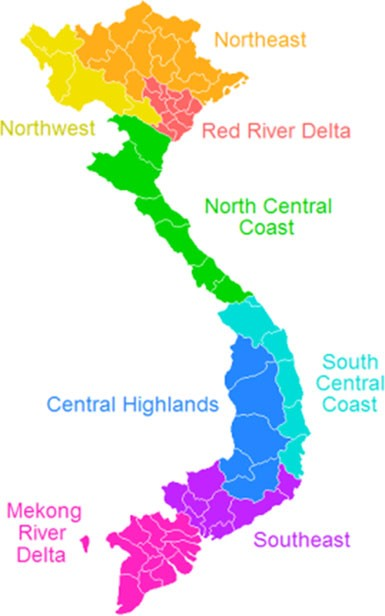
\includegraphics[width = 0.5\textwidth, height = 0.7\textwidth]{pictures/VietnamStatisticalRegions.jpg}
\end{center}
\footnotesize{Source: The illustration is published in \cite{boateng2012GIS}.}
\end{figure}

\section{Model}\label{sec:modelderivation}
This report is a guide on how to use the spatial small open economy dynamic general equilibrium model for climate change and adaptation simulations. In general the model belongs to the class of real business cycle models, because no nominal rigidities are explicitly considered. Nevertheless, it is possible to extend the model to feature also nominal rigidities. The model structure is depicted in Figure \ref{fig:ModelStructure}.
\begin{figure}[h]
\caption{Model Structure}\label{fig:ModelStructure}
\begin{center}
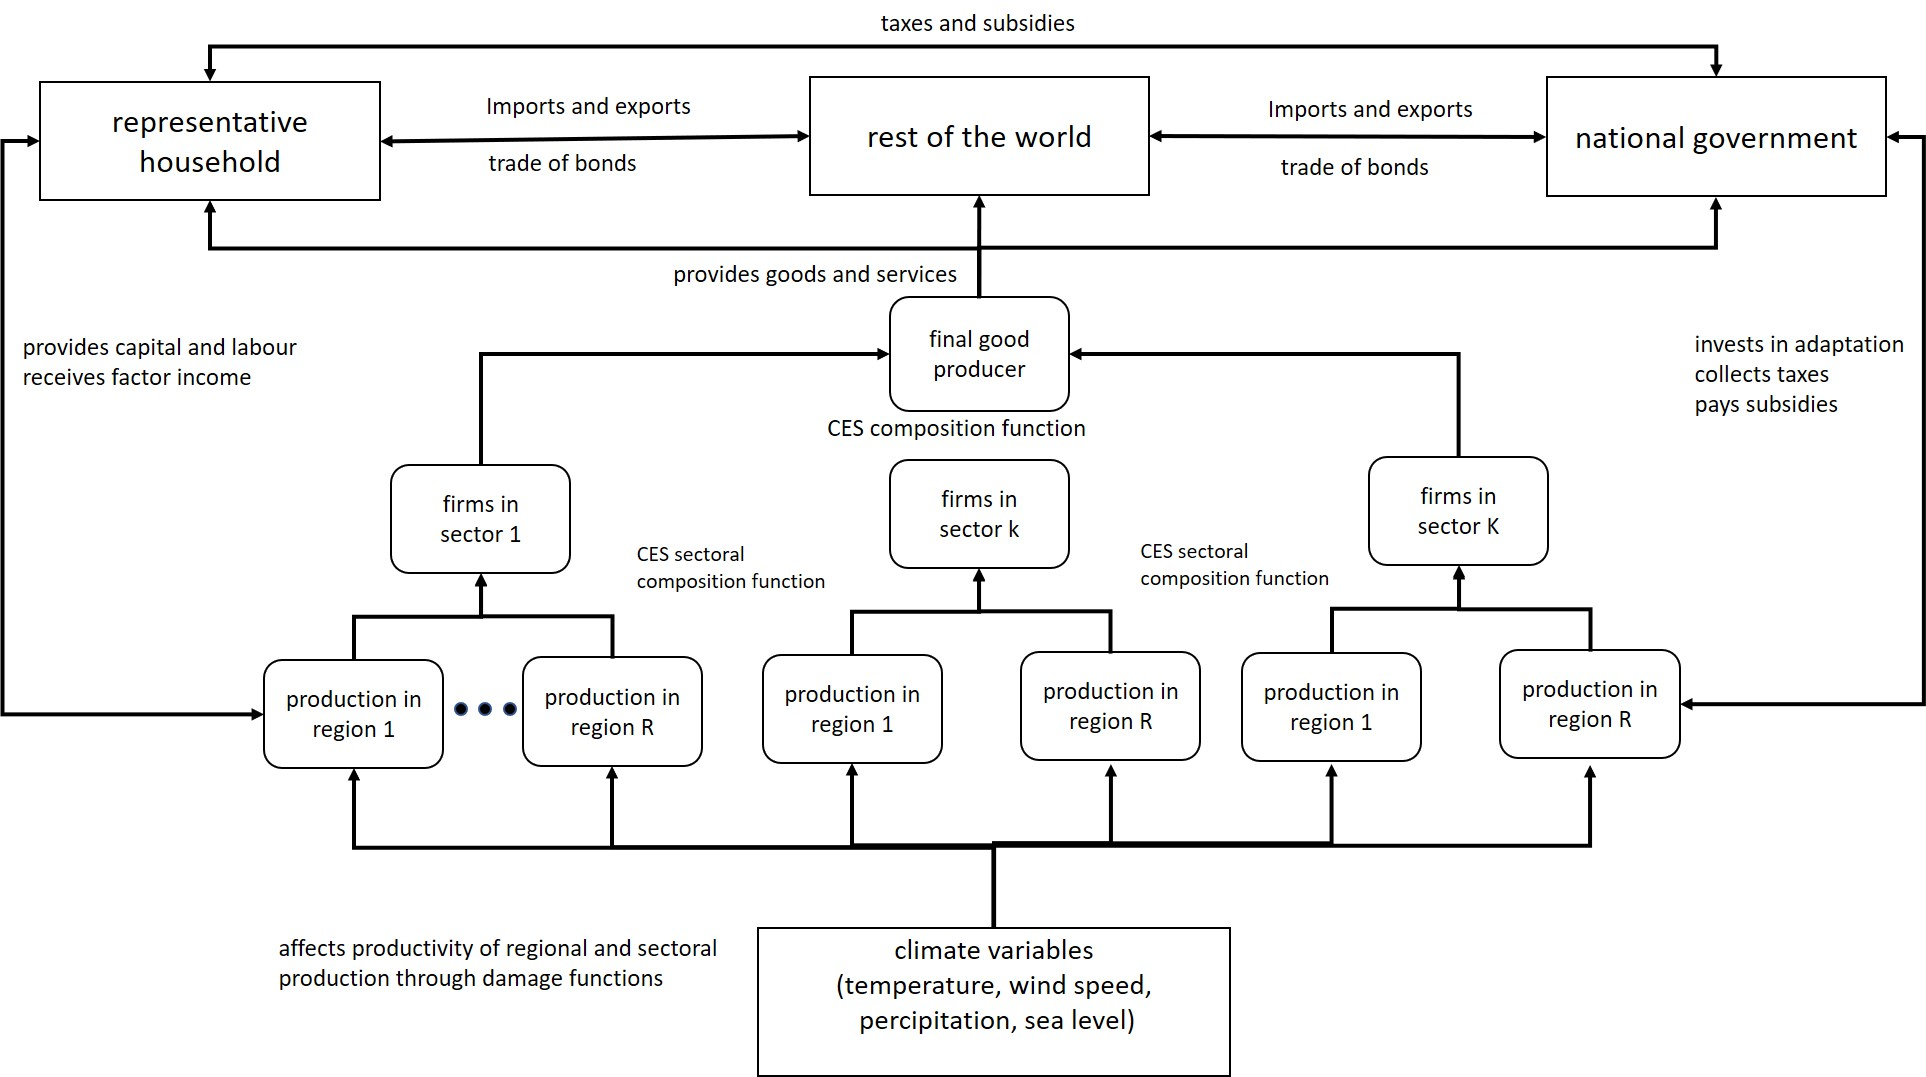
\includegraphics[width = 1\textwidth, height = 0.7\textwidth]{pictures/ModelStructure.jpg}
\end{center}
\footnotesize{Source: own exhibition.}
\end{figure}
Regional climate variables (precipitation, wind speed, temperature and sea level) are exogenous to economic variables. Regional sectoral production functions depend on regional climate variables. The model is meant to reflect small open economies and therefore the climate system is unaffected by the domestic economic system.

The model consists of an arbitrary number of regions ($R$) and sectors ($K$). Regional differentiation is only provided on the supply side and not on the demand side. Representative households consume sectoral goods and supply capital and labour to the firms in the regions. Households also demand goods and services from the rest of the world. Firms use capital and labour to produce sectoral goods with sectoral and regional specific constant elasticity of substitution production functions.

The government collects taxes, consumes and can use its funds to finance adaptation measures for specific regions and sectors. So far, adaptation measures will reduce overall damage by all climate variables at the same time. The effectiveness of government expenditure in one specific region and sector can vary.


Table \ref{tab:listofsymbols} provides a comprehensive list of all variables and parameters. Appendix \ref{app:modelequationsbaseline} reports all equations of the model.

\subsection{Climate variables}
In order to capture the effect of climate change on the economy it is necessary to include climate variables into the model. A small open economy model does not need to include the impact of domestic economic activity on climate variables. Therefore, in contrast to \cite{nordhaus1993optimal} we do not need to model the interaction between economic activity and climate change. Climate variables are independent of other endogenous variables in the model. We explicitly model the regional average annual temperature $T_{r,t}$, the average precipitation $PREC_{r,t}$, the average annual wind speed $W^S_{r,t}$, the sea level $SL_{t}$, cyclones $CYC_{r,t}$ and droughts $DRO_{r,t}$. 
\begin{align}\label{eq:climatevariables}
T_{r,t} = T_{r,0} + \eta_{T,r,t}, \nonumber \\
PREC_{r,t} = PREC_{r,0} + \eta_{PREC,r,t}, \nonumber \\
WS_{r,t} = WS_{r,0} + \eta_{WS,r,t}, \nonumber \\
SL_{t} = SL_{0} + \eta_{SL,r,t}, \nonumber \\
CYC_{r,t} = CYC_{r,0} + \eta_{CYC,r,t}, \nonumber \\
DRO_{r,t} = SL_{r,0} + \eta_{DRO,r,t}. \nonumber \\
\end{align}

The approach in eq.~\ref{eq:climatevariables} allows to specify the evolution of climate variables according to the projections by meteorological models \citep[e.g.][]{stocker2013climate}.

\subsection{Demand}
\subsubsection{Households}
As depicted in Figure \ref{fig:ModelStructure}, the demand side is represented by representative households $h$ providing labour $N$ and capital $K$ to domestic firms $f$. Households maximize discounted utility over an infinite horizon by choosing consumption $C_t(h)$, capital $K_{k,r,t+1}(h)$, investments $I_{k,r,t}(h)$, labour $N_{k,r,t}(h)$ and foreign net wealth $B_{t+1}$ to maximize utility constrained by the budget constraint and the law of motion for sectoral and regional capital. Therefore, the Lagrangian eq.~\ref{eq:hhlagrangian} of the representative household is
\begin{dmath}\label{eq:hhlagrangian}
\sum_{t=0}^{\infty} \beta^{t} \left[ \left(\frac{C_{t}(h)^{1 - \sigma^{C}}}{1 - \sigma^{C}} - \sum_{k=1}^{K} \sum_{r=1}^{R} A^{N}_{k,r,t} \, \phi^{L}_{k,r} \frac{N_{k,r,t}(h)^{1+\sigma^{L}}}{1+\sigma^{L}} \right) 
- \lambda_{t}(h) \left(P_{t} \, C_{t}(h) \, (1 + \tau^{C}) + \sum_{k=1}^{K} \sum_{r=1}^{R} P_{k,r,t} I_{k,r,t}(h) + B_{t+1}(h) - \sum_{k=1}^{K} \sum_{r=1}^{R} (1 - \tau^{N}) \, W_{k,r,t} N_{k,r,t}(h) - \sum_{k=1}^{K} \sum_{r=1}^{R} P_{k,r,t} \, r_{k,r,t} \, (1 - \tau^{K}) \, K_{k,r,t}(h) - S^{f}_{t} \, \phi^{B}_{t} \, (1 + r^{f}_{t} )\, B_{t}(h) \right) 
- \sum_{k=1}^{K} \sum_{r=1}^{R} \lambda_{t}(h) \omega^{I}_{k,r,t}(h) \left\lbrace K_{k,r,t+1} - (1 - \delta - D^K_{k,r,t}) \, K_{k,r,t} - I_{k,r,t} \, \Gamma\left(\frac{I_{k,r,t}}{I_{k,r,t-1}}\right) \right\rbrace \right].
\end{dmath}
Households receive utility by consuming goods, where the intertemporal elasticity of consumption is defined by $\sigma^{C}$. Disutility from labour is sector and region specific $\phi^{L}_{k,r}$, the inverse Frisch elasticity $\sigma^{L}$ is identical for all sectors and regions. Households spent money either on consumption goods $P_t \, C_t(h) \, (1 + \tau^{C})$, regional and sector specific investment $P_{k,r,t} I_{k,r,t}(h)$ or they can lend money $B_{t+1}(h)>0$ to foreing investors. It is also possible that domestic households borrow money from international investors $B_{t+1}(h)<0$. They receive income from labour $W_{k,r,t} \, N_{k,r,t}(h) \, (1 - \tau^{L})$, capital renting $P_{k,r,t} \, r_{k,r,t} \, K_{k,r,t}(h) \, (1 - \tau^{K})$ and interest payments on lent money $B_{t}(h)>0$ or have to pay interest on borrowed money $B_{t}(h)<0$. The first order conditions to the problem are the behavioural equations. Following the literature, we replace the Lagrange multiplier $\lambda_{t}$ by the marginal utility of consumption $\frac{C_{t}(h)^{-\sigma^{C}}}{P_{t}\, (1 + \tau^C)}$ derived from the first order condition (FOC) of the above problem with respect to (w.r.t.) consumption. Households supply labour according to the FOC w.r.t. labour eq.~\ref{eq:hhlaboursupply} for each sector and region depending on the wage $W_{k,r,t}$ and the marginal disutility of labour for the specific sector and region
\begin{dmath}\label{eq:hhlaboursupply}
\phi^{L}_{k,r} \, A^{N}_{k,r,t} \, N_{k,r,t}(h)^{\sigma^{L}} = \lambda_{t}(h) \, W_{k,r,t} \, (1 - \tau^{N}).
\end{dmath}
Households also need to decide how much of their income they want to consume or invest into capital. The famous Euler equation eq.~\ref{eq:hhfoccapital} is obtained by taking the first derivative of the Lagrangian w.r.t. sector and region specific capital
\begin{dmath}\label{eq:hhfoccapital}
\lambda_{t+1}(h) \, \beta \, \left(P_{k,r,t+1} \, r_{k,r,t+1} \, (1 - \tau^K) + (1 - \delta - D^{K}_{k,r,t+1}) \, \omega^{I}_{k,r,t+1} \right) = \lambda_{t}(h) \, \omega^{I}_{k,r,t}.
\end{dmath}

Further, households also face investment adjustment cost $\Gamma(\frac{I_{k,r,t}}{I_{k,r,t-1}}) = 3 - exp\left\lbrace\sqrt{\phi^{K}/2}\left(\frac{I_{k,r,t}}{I_{k,r,t-1}}-1\right\rbrace\right) - exp\left\lbrace-\sqrt{\phi^{K}/2}\left(\frac{I_{k,r,t}}{I_{k,r,t-1}}-1\right)\right\rbrace$, which are sector and region specific. The specification of the investment adjustment cost function is the same as proposed and estimated by \cite{christiano2014risk} for the US.  The marginal value of sectoral and regional investment $\omega^{I}_{k,r,t}$ is determined by

\begin{dmath}\label{eq:hhfocinvestment}
P_{k,r,t} \, \lambda_{t}(h) = \lambda_{t}(h) \, \omega^{I}_{k,r,t} \, \left(\Gamma(\frac{I_{k,r,t}}{I_{k,r,t-1}}) - \frac{\partial \Gamma(\frac{I_{k,r,t}}{I_{k,r,t-1}})}{\partial I_{k,r,t}} \, \frac{I_{k,r,t}}{I_{k,r,t-1}} \right) + \beta \lambda_{t+1}(h) \, \omega^{I}_{k,r,t+1} \, \frac{\partial \Gamma(\frac{I_{k,r,t+1}}{I_{k,r,t}})}{\partial I_{k,r,t}} \, \left(\frac{I_{k,r,t+1}}{I_{k,r,t}}\right)^2
\end{dmath}

\subsubsection{Rest of the world}
Households have access to the international financial market to purchase and sell internationally-traded bonds. However, we only consider net foreign positions 

\begin{dmath}\label{eq:hhfocbonds}
\lambda_{t+1} \, \beta \, S^{f}_{t+1} \, \phi^{B}_{t+1} \left(1+{{r^{f}}_{t+1}}\right) = \lambda_{t} \\
\end{dmath}
with effective exchange rate $S^f$ and the world interest rate $r^f$.
The required interest rate is above the world interest rate if the foreign debt ($B_{t+1}<0$)/ foreign claims ($B_{t+1}>0$) relative to GDP increases/decreases and future net exports relative to GDP will decrease. 
\begin{dmath}
\phi^{B}_{t+1} = exp \left(-\phi^B \,(S^{f}_{t+1} \, r^{f}_{t+1} \, \frac{B_{t+1}}{Y_{t+1}}+\frac{NX_{t+1}}{Y_{t+1}})\right)
\end{dmath}
Here we introduce $\phi^{B}_{t+1}$ to ensure stability of the system as discussed in \cite{schmitt2003closing}.


\subsubsection{Government}

We are interested in different policy measures taken by the government to adapt to a new climate regime. Government behaviour is not a result of an optimization problem. The government collects taxes from consumption $\tau^{C} \, C_{t}$, labour income $\sum_{k}^{K} \sum_{r}^{R} \, (\tau^{N} + \tau_{k,r,t}^{N}) \, W_{k,r,t} \, N_{k,r,t} \, Pop_{t}$ and capital income $\sum_{k}^{K} \sum_{r}^{R} \, (\tau^{K} + \tau_{r,k,t}^{K}) \, P_{k,r,t} \, r_{k,r,t} \, K_{k,r,t}$. In order to finance its activities the government can borrow loans from the rest of the world $B^{G}_{t+1}<0$ and has to repay loans and interest from the previous period denominated in foreign currency $(1 + r^{f}_{t})$ identical to the interest rates paid by households. The government budget constraint boils down to eq.~\ref{eq:GovBudget}.
\begin{align}\label{eq:GovBudget}
G_{t} + \sum_{k}^{K} \sum_{r}^{R} G^{A}_{k,r,t} + B^G_{t+1} =& \sum_{k}^{K} \sum_{r}^{R} \, \left\lbrace (\tau^{K} + \tau_{r,k,t}^{K}) \, P_{k,r,t} \, r_{k,r,t} \, K_{k,r,t} + (\tau^{N} + \tau_{k,r,t}^{N}) \, W_{k,r,t} \, N_{k,r,t} \, Pop_{t} \right\rbrace \nonumber \\
& + (1 + r^{f}_{t}) \, S^{f}_{t} \phi^{B}_{t} \, B^G_{t}
\end{align}

Government expenditures can be used to finance adaptation measures in specific sectors and regions $G^{A,z}_{k,n,t}$ against different climate variables $z \in \{WS,PREC,T,CYC,DRO,SL\}$. The effectiveness of adaptation measures might also depend on previous expenditures of the government. Therefore, we consider capital stocks $K^{A,z}_{k,r,t+1}$ financed by expenditures on adaptation measures. The depreciation rate $\delta_{K^{A,z},k,r}$ defines necessary maintenance costs, which are assumed to be proportional to the capital stock.  

Government expenditures on adaptation measures, taxes on regional and sectoral capital expenditure, and government debt are independent of other variables or to formulate it differently are discretionary. This allows us to evaluate different policy paths for the future and to model the variables by exogenous processes as stated in eq.~\ref{eq:GovExpenditure}.
\begin{align}\label{eq:GovExpenditure}
K^{A,z}_{k,r,t+1} = \eta^{A,z}_{k,r,t} \nonumber \\
K^{A,z}_{k,r,t+1} = (1 - \delta_{K^{A,z},k,r}) \, K^{A,z}_{k,r,t} + G^{A,z}_{k,r,t} \nonumber \\
\tau^{K}_{k,r,t} = \tau^{K}_{k,r,0} + \eta^{\tau^{K}}_{k,r,t} \nonumber \\
\tau^{N}_{k,r,t} = \tau^{N}_{k,r,0} + \eta^{\tau^{N}}_{k,r,t} \nonumber \\
B^G_{t+1} = B^G_{0} + \eta^{B^{G}}_{t}
\end{align} 

\subsubsection{Resource constraint}

Households and government use domestic final goods $Y_t$ produced by firms for consumption, investment and for exports $X_{t}$ and can also use imports $M_t$ for consumption and investment. This gives rise to the well known resource constraint or the expenditure approach to define GDP 
\begin{align}
Y_{t} = C_{t} + I_{t} + G_{t} + \underbrace{X_{t} - M_{t}}_{NX_{t}}
\end{align}

The aggregation of the budget constraints of the representative households also states that positive net exports are used to increase net financial wealth to the rest of the world.
\begin{align}
NX_t = B_{t+1} - (1 + r^{f}_{t}) S^{f}_{t} \phi^B_{t} B_{t}
\end{align}

\subsection{Production}

Households demand final domestic goods $Y_{t}$ combining goods from different sectors $Y_{k,t}$ using a CES production function. They minimize expenditures subject to the production function
\begin{align}
\underset{Y_{k,t}}{\mathrm{min}} & \sum_{k} Y_{k,t} \, P_{k,t} \\ 
Y_{t} &= \left(\sum_{k} {\omega^{Q}_{k}}^{\frac{1}{\eta^Q}} Y_{k,t}^{\frac{\eta^Q-1}{\eta^Q}} \right)^{\frac{\eta^Q}{\eta^Q-1}}
\end{align}

Therefore, the demand for sectoral products correspond to the first order conditions of the above optimization problem. The Lagrange multiplier is the price level $P_{t}$ of domestic products. 
\begin{align}
\frac{P_{k,t}}{P_{t}} &= {\omega^{Q}_{k}}^{\frac{1}{\eta^Q}} \left(\frac{Y_{k,t}}{Y_{t}}\right)^{\frac{-1}{\eta^Q}}
\end{align}

In order to model regional economic activity we further decompose the production process on a regional level. One can either think about this approach as modeling the optimization problem of a representative firm operating in one sector on a national level allocating production activity across the nation. Another way is to consider that households make direct purchases from regional operating firms in one sector. In this case the following optimization problem would be part of the above optimization problem. 
\begin{align}
\underset{Y_{k,r,t}}{\mathrm{min}} & \sum_{k} Y_{k,r,t} \, P_{k,r,t} \\ 
Y_{k,t} &= \left(\sum_{k} {\omega^{Q}_{k,r}}^{\frac{1}{\eta^Q_{k}}} Y_{k,r,t}^{\frac{\eta^Q_{k}-1}{\eta^Q_{k}}} \right)^{\frac{\eta^Q_{k}}{\eta^Q_{k}-1}}
\end{align}

Demand for sectoral and regional products correspond to the first order conditions of the above optimization problem. The Lagrange multiplier is the sectoral price level $P_{k,t}$ of domestic products. 
\begin{align}
\frac{P_{k,r,t}}{P_{k,t}} &= {\omega^{Q}_{k,r}}^{\frac{1}{\eta^{Q}_{k}}} \left(\frac{Y_{k,r,t}}{Y_{k,t}}\right)^{\frac{-1}{\eta^{Q}_{k}}}
\end{align}

At the regional and sectoral level are representative firms maximizing profits using capital $K_{k,r,t}$ and labour $L_{k,r,t} = N_{k,r,t} \, Pop_{t}$ provided by households to produce products. They charge a price $P_{k,r,t}$ for their products and have to pay households wages $W_{k,r,t}$, interest on rented capital $P_{r,k,t} \, r_{r,k,t}$, taxes related to the wage bill $\tau^{N}_{r,k,t}$ and on capital expenditure $\tau^{K}_{r,k,t}$.  Representative firms have access to a regional and sector specific constant elasticity of substitution production function. The productivity of capital and labour of a firm in one sector and region depends on the climate variables, and the adaption measures by the government represented by a damage function affecting total factor productivity $A_{k,r,t}$ by $D_{k,r,t} = D_{k,r}\left(T_{r,t}, \, PREC_{r,t}, \, WS_{r,t}, \, SL_{r,t}, \, CYC_{r,t}, \, DRO_{r,t}, \, G^{A}_{r,k,t} \right)$.  Further, we explicity differentiate between climate induced damages affecting labour productivity $D_{N,k,r,t}$ and capital depreciation $D_{K,k,r,t}$. As in \cite{nordhaus1993optimal}, we assume a polynomial functional form of the damage functions, but the damages are different across regions and sectors (eq.~\ref{eq:Damages}).

\begin{align}
{{D_{k,r}}_{t}}=& \Big\lbrace \nonumber \\
& (\underbrace{{{a_{T,1,k,r}}} \, {{T_{r}}_{t}}+{{a_{T,2,k,r}}}\, \left({T_{r}}_{t}\right)^{a_{T,3,k,r}}}_{\mbox{impact of temperature}})  \, \underbrace{exp(-\phi^{G^{A,T}}_{k,r} K^{A,T}_{k,r,t})}_{\mbox{impact of adaptation}} \,  \nonumber \\
+ & (\underbrace{{{a_{SL,1,k,r}}}\, {{SL}_{t}}+{{a_{SL,2,k,r}}}\, \left({SL}_{t}\right)^{{{a_{SL,3,k,r}}}}}_{\mbox{impact of sea level}})   \, \underbrace{I(SL > \frac{K^{A,SL}_{k,r,t}}{\phi^{G^{A,SL}}_{k,r}})}_{\mbox{impact of adaptation}} \nonumber \\
+ & (\underbrace{{{a_{WS,1,k,r}}}\, {{WS_{r}}_{t}}+{{a_{WS,2,k,r}}}\, \left({WS_{r}}_{t}\right)^{{{a_{WS,3,k,r}}}}}_{\mbox{impact of wind speed}}) \, \underbrace{exp(-\phi^{G^{A,WS}}_{k,r} K^{A,WS}_{k,r,t})}_{\mbox{impact of adaptation}} \nonumber \\
+ & (\underbrace{{{a_{PREC,1,k,r}}} \, {{PREC_{r}}_{t}}+{{a_{PREC,2,k,r}}}\, \left({PREC_{r}}_{t}\right)^{{{a_{PREC,3,k,r}}}}}_{\mbox{impact of precipitation}}) \, \underbrace{exp(-\phi^{G^{A,PREC}}_{k,r} K^{A,PREC}_{k,r,t})}_{\mbox{impact of adaptation}} \nonumber \\
+ & (\underbrace{{{a_{CYC,1,k,r}}}\, {{CYC_{r}}_{t}}+{{a_{CYC,2,k,r}}}\, \left({CYC_{r}}_{t}\right)^{{{a_{CYC,3,k,r}}}}}_{\mbox{impact of cyclones}}) \, \underbrace{exp(-\phi^{G^{A,CYC}}_{k,r} K^{A,CYC}_{k,r,t})}_{\mbox{impact of adaptation}}  \nonumber \\ 
+ & (\underbrace{{{a_{DRO,1,k,r}}} \, {{DRO_{r}}_{t}}+{{a_{DRO,2,k,r}}}\, \left({DRO_{r}}_{t}\right)^{{{a_{DRO,3,k,r}}}}}_{\mbox{impact of droughts}}) \, \underbrace{exp(-\phi^{G^{A,DRO}}_{k,r} K^{A,DRO}_{k,r,t})}_{\mbox{impact of adaptation}}  \nonumber \\
&\Big\rbrace. \label{eq:Damages} \\
{{D^{N}_{k,r}}_{t}}=& \Big( \nonumber \\
&\underbrace{{{a^{N}_{T,1,k,r}}} \, {{T_{r}}_{t}}+{{a^{N}_{T,2,k,r}}}\, \left({T_{r}}_{t}\right)^{a^{N}_{T,3,k,r}}}_{\mbox{impact of temperature}} + 
\underbrace{{{a^{N}_{SL,1,k,r}}}\, {{SL}_{t}}+{{a^{N}_{SL,2,k,r}}}\, \left({SL}_{t}\right)^{{{a^{N}_{SL,3,k,r}}}}}_{\mbox{impact of sea level}} \nonumber \\
+ & \underbrace{{{a^{N}_{WS,1,k,r}}}\, {{WS_{r}}_{t}}+{{a^{N}_{WS,2,k,r}}}\, \left({WS_{r}}_{t}\right)^{{{a^{N}_{WS,3,k,r}}}}}_{\mbox{impact of wind speed}} 
+ (\underbrace{{{a^{N}_{PREC,1,k,r}}} \, {{PREC_{r}}_{t}}+{{a^{N}_{PREC,2,k,r}}}\, \left({PREC_{r}}_{t}\right)^{{{a^{N}_{PREC,3,k,r}}}}}_{\mbox{impact of precipitation}}) \,  \nonumber \\
+ & \underbrace{{{a^{N}_{CYC,1,k,r}}}\, {{CYC_{r}}_{t}}+{{a^{N}_{CYC,2,k,r}}}\, \left({CYC_{r}}_{t}\right)^{{{a^{N}_{CYC,3,k,r}}}}}_{\mbox{impact of cyclones}}
+ \underbrace{{{a^{N}_{DRO,1,k,r}}} \, {{DRO_{r}}_{t}}+{{a^{N}_{DRO,2,k,r}}}\, \left({DRO_{r}}_{t}\right)^{{{a^{N}_{DRO,3,k,r}}}}}_{\mbox{impact of droughts}} \nonumber \\
&\Big). \label{eq:DamagesLabour} \\
{{D^{K}_{k,r}}_{t}}=& \Big( \nonumber \\
&\underbrace{{{a^{K}_{T,1,k,r}}} \, {{T_{r}}_{t}}+{{a^{K}_{T,2,k,r}}}\, \left({T_{r}}_{t}\right)^{a^{K}_{T,3,k,r}}}_{\mbox{impact of temperature}}+ \underbrace{{{a^{K}_{SL,1,k,r}}}\, {{SL}_{t}}+{{a^{K}_{SL,2,k,r}}}\, \left({SL}_{t}\right)^{{{a^{K}_{SL,3,k,r}}}}}_{\mbox{impact of sea level}} \nonumber \\
+ & \underbrace{{{a^{K}_{WS,1,k,r}}}\, {{WS_{r}}_{t}}+{{a^{K}_{WS,2,k,r}}}\, \left({WS_{r}}_{t}\right)^{{{a^{K}_{WS,3,k,r}}}}}_{\mbox{impact of wind speed}}
+ \underbrace{{{a^{K}_{PREC,1,k,r}}} \, {{PREC_{r}}_{t}}+{{a^{K}_{PREC,2,k,r}}}\, \left({PREC_{r}}_{t}\right)^{{{a^{K}_{PREC,3,k,r}}}}}_{\mbox{impact of precipitation}} \nonumber \\
+ & \underbrace{{{a^{K}_{CYC,1,k,r}}}\, {{CYC_{r}}_{t}}+{{a^{K}_{CYC,2,k,r}}}\, \left({CYC_{r}}_{t}\right)^{{{a^{K}_{CYC,3,k,r}}}}}_{\mbox{impact of cyclones}}
+ \underbrace{{{a^{K}_{DRO,1,k,r}}} \, {{DRO_{r}}_{t}}+{{a^{K}_{DRO,2,k,r}}}\, \left({DRO_{r}}_{t}\right)^{{{a^{K}_{DRO,3,k,r}}}}}_{\mbox{impact of droughts}} \nonumber \\
&\Big). \label{eq:DamagesCapital}
\end{align}

Firms in each region and sector have access to a constant elasticity of substitution production function with production factors labour and capital. Eq.~\ref{eq:profitoptim} states the optimization problem of the firm.
\begin{align}\label{eq:profitoptim}
\underset{Y_{k,r,t}, N_{k,r,t}, K_{k,r,t}}{\mathrm{max}} P_{k,r,t} \, Y_{k,r,t} - W_{k,r,t} \, N_{k,r,t} \, Pop_{t} \, (1 + \tau^{N}_{k,r,t}) - r_{k,r,t} \, P_{k,r,t} \, K_{k,r,t} \, (1 + \tau^{K}_{k,r,t})\nonumber \\ 
\mbox{s.t.} \, Y_{k,r,t} = A_{k,r,t} (1 - D_{k,r,t}) \, \left[{\alpha^{N}_{k,r}}^{\frac{1}{\eta^{NK}_{k,r}}} \, \left( A^{N}_{k,r,t} \, (1 - D^{N}_{k,r,t}) \, Pop_{t} \, N_{k,r,t}\right)^{\rho_{k,r}} + {\alpha^{K}_{k,r}}^{\frac{1}{\eta^{NK}_{k,r}}} \, \left(K_{k,r,t}\right)^{\rho_{k,r}}\right]^{\frac{1}{\rho_{k,r}}}, \nonumber \\
\mbox{ where } \rho_{k,r} = \frac{\eta^{NK}_{k} - 1}{\eta^{NK}_{k}}.
\end{align}

Demand for production factors are given by the first order condition of the above optimization problem. The Lagrange multiplier is equal to the price charged by companies. 

\begin{align}\label{eq:focfirm}
\frac{W_{k,r,t}}{P_{k,r,t}}  \, (1 + \tau^{N}_{k,r,t}) = {\alpha^{N}_{k,r}}^{\frac{1}{\eta^{NK}_{k,r}}} \, \left(A_{k,r,t} \, (1 - D_{k,r,t}) \, A^N_{k,r,t} \, (1 - D^N_{k,r,t})\right)^{\rho_{k,r}} \left(\frac{Pop_{t} N_{k,r,t}}{Y_{k,r,t}}\right)^{-\frac{1}{\eta^{NK}_{k,r}}} \nonumber \\ 
r_{k,r,t} \, (1 + \tau^{K}_{k,r,t}) = {\alpha^{K}_{k,r}}^{\frac{1}{\eta^{NK}_{k,r}}} \, \left(A_{k,r,t} \, (1 - D_{k,r,t})\right)^{\rho_{k,r}}\left(\frac{K_{k,r,t}}{Y_{k,r,t}} \right)^{-\frac{1}{\eta^{NK}_{k,r}}} \\ 
\end{align}

We use the more general case of the CES production function rather than the more commonly used Cobb-Douglas production function. The parameter $\eta^{NK}_{k,r}$ allows us to control the response of capital and labour demand to temporary productivity shocks. Temporary productivity shocks are in our set-up also weather extremes. Cyclones can destroy the capital stock. Firms can either substitute caital using more labour in the period, e.g. using more labour to replace tractors. Or they need to layoff workers because they are useless without machines, e.g. destruction of factories. The parameter $\eta^{NK}_{k,r}$ allows to specify the reaction of firms according to the data.

\subsection{Rest of the world}

The demand for domestic exports and foreign imports is not explicitly modeled in this version of the model. We assume that net exports follow an auto-regressive process of order one and that the long-run value of net exports depend on the long-run development of gross domestic product. We therefore assume that imports and exports will grow at the same speed as GDP. Sluggish adjustments in export and import behaviour of companies is captured by an auto-regressive process. 
\begin{align}
NX_{t} = \rho^{NX} \, NX_{t-1} + (1 - \rho^{NX}) \omega^{NX} P_{t} \, Y_{t} \, exp\left({{\eta_{NX}}_{t}}\right)
\end{align}

The effective exchange rate $S^f_{t}$ and the world interest rate $r^{f}_{t}$ determine how much governments and households have to pay back in domestic currency as net lender or how much they receive as net borrower to the rest of the world. Here the world interest rate is independent of domestic developments and only the effective exchange rate adjusts according to eq.~\ref{eq:hhfocbonds}.

\subsection{Model extension: intermediate consumption and sectoral trade} 
Table \ref{tab:listofsymbolsextension1} provides a list of all additional variables and parameters included for the extension. Appendix \ref{app:modelequationsextension1} reports all additional and modified equations associated with the respective extension.

In order to consider the impact of climate change on exports and imports, we need to extend the model to feature sectoral exports $X_{k,t}$ and imports $M_{k,t}$. It is also necessary to include intermediate consumption $Q^{I}_{k,r,t}$ by firms to ensure that the model can be calibrated to match export and import ratios for different sectors. In contrast to the baseline version imports are used to produce final domestically used output $Q^U_t$. The later is provided by a representative firm using domestic output from different sectors and regions $Q^{D}_{k,t}$ and sectoral imports. Imports and domestic products from different sectors are combined using a CES production function. The production function of the firm is a nested CES function:
\begin{align}
Q^U_t = \left((1 - \omega^{F})^{\frac{1}{\eta^{F}}} \, {Q^D_t}^{\rho^F} + {\omega^{F}}^{\frac{1}{\eta^{F}}} \, {M_t}^{\rho^F}\right)^{\frac{1}{\rho^F}}, \mbox{where } \rho^{F} = \frac{\eta^F - 1}{\eta^F} \label{eq:cesfinal}\\
M_t = \left(\sum_{k}^{K}{\omega^{M}_{k}}^{\frac{1}{\eta^{M}}} \, {M_{k,t}}^{\rho^M}\right)^{\frac{1}{\rho^M}}, \mbox{where } \rho^{M} = \frac{\eta^M - 1}{\eta^M} \label{eq:imports} \\
Q^D_t = \left(\sum_{k}^{K}{\omega^{Q}_{k}}^{\frac{1}{\eta^{Q}}} \, {Q^D_{k,t}}^{\rho^Q}\right)^{\frac{1}{\rho^Q}}, \mbox{where } \rho^{Q} = \frac{\eta^Q - 1}{\eta^Q} \label{eq:domesticusedoutput} \\
Q^{D}_{k,t} = Q_{k,t} - X_{k,t} \nonumber \\ 
Q_{k,t} = \left(\sum_{k}^{K}{\omega^{Q}_{k,r}}^{\frac{1}{\eta^{Q}_{k}}} \, {Q_{k,r,t}}^{\rho^Q_{k}}\right)^{\frac{1}{\rho^Q_{k}}}, \mbox{where } \rho^{Q}_{k} = \frac{\eta^Q_{k} - 1}{\eta^Q_{k}} \nonumber 
\end{align}

Prices of sectoral imports $P^{M}_{k,t}$ are exogenous (eq.~\eqref{eq:importprices}) as well as the export demand (eq.~\eqref{eq:exportsdemand}) for domestic produced sectoral products. The optimization problem of the final goods producer can be split up into different parts. According to eq.~\eqref{eq:cesfinal} they first choose the amount of imports (eq.~\eqref{eq:demandimports}) and domestically used and produced products (eq.~\eqref{eq:demanddomesticoutput}). In the next layer the final goods producer minimizes costs for a given level of imports (eq.~\eqref{eq:imports}) and domestically used and produced output (eq.~\eqref{eq:domesticusedoutput}). This leads to demand functions for sectoral domestic output (eq.~\eqref{eq:demandsectoraloutput}) and sectoral imports (eq.~\eqref{eq:demandsectoralimports}).

Further, imports and domestic production are used to consume, invest and for intermediate goods $Q^{I}_{k,r,t}$ in the domestic production process. Therefore, firms are using labour and capital, but also intermediate input to produce goods and services. The production function of firms operating in different regions is now modified to feature another layer of the CES production function. The firm is now maximizing profits combining value-added $Y_{k,r,t}$ and intermediate products $Q^{I}_{k,r,t}$ to produce output $Q_{k,r,t}$. They sell their products under prefect competition for the price $P^{D}_{k,r,t}$. The optimization problem is 
\begin{align}
\underset{Q^{I}_{k,r,t}, \, Y_{k,r,t}}{\mathrm{min}} P^{D}_{k,r,t} \, Q_{k,r,t} - P_{t} \, Q^{I}_{k,r,t} - P_{k,r,t} \, Y_{k,r,t} \nonumber \\
Q_{k,r,t} = \left({\omega^{Q^{I}}_{k,r}}^{\frac{1}{\eta^{I}_{k,r}}} \, {Q^{I}_{k,r,t}}^{rho^{I}_{k,r}} + (1 - \omega^{Q^{I}}_{k,r})^{\frac{1}{\eta^{I}_{k,r}}} \, {Y_{k,r,t}}^{\rho^{I}_{k,r}} \right)^{\frac{1}{\rho^I_{k,r}}}, \mbox{where } \rho^I_{k,r} = \frac{\eta^{I}_{k,r} - 1}{\eta^{I}_{k,r}}
\end{align}

Therefore, we obtain equations determining the demand for value added (eq.~\eqref{eq:demandva}) and intermediate products (eq.~\eqref{eq:demandinput}) by one sector in a region depending on the relative prices of labour, capital and intermediate products.
\begin{align}
\frac{{{P_{k,r}}_{t}}}{{P^{D}_{k,r,t}}}=\left(1 - {\omega^{Q^{I}}_{k,r}}\right)^{\frac{1}{{{\eta^{I}_{k}}}}} \, \left(\frac{Y_{k,r,t}}{Q_{k,r,t}}\right)^{\frac{\left(-1\right)}{{{\eta^{I}_{k}}}}} \label{eq:demandva}\\
\frac{{P_{t}}}{{P^{D}_{k,r,t}}}={\omega^{Q^{I}}_{k,r}}^{\frac{1}{{{\eta^{I}_{k}}}}} \, \left(\frac{Q^{I}_{k,r,t}}{Q_{k,r,t}}\right)^{\frac{\left(-1\right)}{{{\eta^{I}_{k}}}}} \label{eq:demandinput}
\end{align}

Net exports (eq.~\eqref{eq:netexports}) are now the difference between aggregate export expenditures $P^{D}_{t} X_{t}$ and aggregate import expenditures $P^{M}_{t} M_{t}$. The resource constraint now equates total domestic production with domestic consumption, investment, government consumption, net exports and intermediate products (eq.~\eqref{eq:resourceconstraint}). Gross value added is total domestic output less total intermediate consumption.

\subsection{Model extension: energy consumption} 
Table \ref{tab:listofsymbolsextension2} provides a list of all additional variables and parameters included for the extension. Appendix \ref{app:modelequationsextension2} reports all additional and modified equations associated with the respective extension.

To model the impact of mitigation policy on the economy we define an energy sector $k^{E}$. We add two new layers to the production function in the energy sector. The energy sector uses intermediate products $Q^{I}_{k^{E},r,t}$ and a composite energy product $E_{k,r,t}$ to produce a composite intermediate product $Q^{I,E}_{k,r,t}$ (eq.~\eqref{eq:energyintermediatecomposite}). The composite energy input is a combination of different energy carriers $c \in \{1, \dots, EC\}$ using a CES production function (eq.~\eqref{eq:energycomposite}). The price of an energy carrier is the same across regions and exogenous to other variables (eq.~\eqref{eq:priceenergycarrier}). Aggregate consumption of energy carriers (eq.~\eqref{eq:energycarrieraggregate}) is necessary to compute emissions associated with different energy carriers. Total  intermediate input $Q^{I}_{t}$ expenditures is the sum over all intermediate inputs demanded by different sectors including expenditures on energy carriers (eq.~\eqref{eq:aggregationintermediateinputswithenergy}).

\section{Scenario Analysis}

For simulations it is necessary to specify a direct mapping between sectors in the model and the available data. The analysis in the following paragraphs will differentiate between three economic sectors: 
\begin{enumerate}
	\item A - agriculture, forestry and fishing
	\item B-F: industrial sectors (mining and quarrying, manufacturing, electricity, gas, stream and air conditioning supply, water supply, sewerage, waste management and remediation activities) and construction
	\item G-T: services
\end{enumerate}

It is also necessary to define the regions. Therefore, we will explicitly model three regions: 
\begin{enumerate}
	\item Mekong River Delta
	\item Red River Delta
	\item North Central and Central Coast, Southeast, Central Highlands, Northern Midlands and Mountains
\end{enumerate}

We calibrate the model to reflect the economic structure of Vietnam for the year 2016. The year 2016 is our base year, because the latest supply and use table is available for this year. We calibrate the production function parameters $\alpha^{K}_{k,r,n}, \, \alpha^{N}_{k,r,n}$ such that we match for a given elasticity of substitution $\eta^{NK}_{k,r}$ the observed share of the wage bill on gross value added $\frac{W_{k,r,0} \, N_{k,r,0}}{P_{k,r,0} \, Y_{k,r,0}}$ and ensure a correct accounting of factor income by economic activity. Further, we calibrate the sectoral composition production function parameters $\omega^{Q}_{k,r},\, \omega^{Q}_{k}$ for a given elasticity of substitutions $\eta^{Q}, \, \eta^{Q}_{k}$ to meet the initial gross value added shares $\phi^{Y}_{k,r,0} = \frac{P_{k,r,0} \, Y_{k,r,0}}{P_{0} \, Y_{0}}$ for the year 2016.

A scenario defines paths for variables exogenous to the economic system. In the standard version of the model we need to define how exogenous total factor productivity $\eta_{A,k,r,t}$, labour productivity $\eta^{A^N}_{k,r,t}$, climate variables $\{\eta^{T}_{r,t},\, \eta^{PREC}_{r,t},\, \eta^{WS}_{r,t},\, \eta^{CYC}_{r,t},\, \eta^{DRO}_{r,t},\, \eta^{SL}_{t}\}$, population $\eta^{Pop}_{t}$, price level $\eta^{P}_{t}$, taxes  $\eta^{\tau^{K,N}}_{k,r,t},\, \eta^{\tau^{K,N}}_{t},\, \eta^{\tau^{C}}_{t}$, the government deficit $\eta^{BG}_{t}$, adaptation measures $\eta^{G^{A}}_{k,r,t}$ and the trade balance $\eta^{NX}_{t}$ evolve over time. 

\subsection{Baseline}

Vietnam is a developing economy with a GDP per capita in constant 2010 US Dollar of 1,752 USD equivalent to roughly 4 percent of Japan's GDP per capita in 2016. Japan was the first Asian country becoming a developed economy in the 20th century. We will use the development of the Japanese economy in the 20th century as a benchmark for a counter-factual development of Vietnam without climate change in the 21st century. Japan is the best benchmark among other developed economies, which are either the United States of America or countries from Europe. In contrast to China still considered a developing economy, Vietnam and Japan have a similar population size. Japan's GDP grew annually from 1960 to 2018 by 3 percent according to the World Bank. In the Baseline scenario Vietnam's geometric average annual growth rate will be 4 percent for the next century.

It is common for developing economies to face also a change in the composition of their economic structure. The agricultural sector in Vietnam is still an important employer (40\% of all employees work in the agricultural sector) and is responsible for roughly 15\% of total gross value added in Vietnam. In developed countries (e.g. Japan, Germany, United Kingdom etc.) the share of agriculture on total gross value added is approximately 1\% and the share of employees is roughly the same. Services contribute 64\% and mining, manufacturing, water supply and waste management, energy supply, and construction contribute 35\% to GDP. We therefore determine sectoral total productivity shocks $\eta_{A,k,r,t}$ to match an assumed new long-run composition of gross value added by economic activity $\phi^{Y}_{k,r,T} = \frac{P_{k,r,T} \, Y_{k,r,T}}{P_{T} \, Y_{T}}$. We also define the long-run development on the labour market. The long-run development of labour productivity $\eta_{A^{N},k,r,t}$ ensures that employment shares $\phi^{Y}_{k,r,T} = \frac{Pop_{T} \, N_{k,r,T}}{Pop_{T} \, N_{T}}$ will converge to observed shares for other industrial countries. The evolution of sector specific labour productivity and total factor productivity is determined such that the initial simulated sectoral growth rates of labour share $g^{N}_{k,r,1} = \frac{N_{k,r,1}/N_{1}}{N_{k,r,0}/N_{0}}$ and real gross value added $g^{Y}_{k,r,1} = \frac{Y_{k,r,1}}{Y_{k,r,0}}$ match the observed growth rates of different sectors in Vietnam over the last decade. Growth rates follow an auto-regressive process of order one, where the auto-correlation parameter is determined such that growth rates are approximately zero after 120 periods. We ensure that the exogenous evolution of sectoral labour and total factor productivity is completed after 120 periods.

The evolution of the population is given by the projection of the GSO. The GSO published four different projections with different fertility rates of the Vietnamese population. We use the medium variant population projection. The population is expected to grow from roughly 95 million people in 2016 to 108 million people by 2050. After 2050 the population stays constant. In our simulation we do not consider potential feedback between the economic development of Vietnam and the development of the population. Potential interdependence between the population and climate change through higher mortality caused by weather extremes (e.g. droughts, heat waves, cyclones) is not considered. It is hard to find studies on the effects of temperature increases on the services sector regarding TFP. Therefore, we will assume that the productivity of the services sector is unaffected by annual average increase in temperature.

\subsection{Temperature}

Average annual temperature change will not exceed 6 degree Celsius with a probability of 90\% according to down scaling techniques of the RCP 8.5 scenario from the IPCC conducted by \cite{thuc2016climate}. We consider the upper bound to estimate the maximum expected damage associated with a change in temperature. The average annual temperature will follow a linear trend. According to the results published in \cite{thuc2016climate} the average annual temperature in the Mekong River Delta, Red River Delta, and the remaining regions will increase by 4.4, 5.4, and 5 degree Celsius until the end of the 21st century, respectively. 

To evaluate the impact of climate change on the economy in Vietnam we need to specify the parameters $a_{T,\{1,2,3\},k,r}, \, a^{N}_{T,\{1,2,3\},k,r}, \, a^{K}_{T,\{1,2,3\},k,r}$ of the damage functions. We use the literature to define these parameters. We  assume a linear relationship between total factor productivity of the agricultural sector and a change in temperature. The coefficient $a_{T,1,1,r}$ is set to $0.045$ based on \cite{challinor2014meta} and the other parameters are set to zero for agriculture. \cite{challinor2014meta} report a decline of crop yield of 4.5\% as a response to a one degree Celsius increase in average annual temperature. This is a simplification of a complex causal mechanism between temperature and crop yield. Further, different crops will respond differently to a one degree Celsius increase of temperature. It is possible to explicitly model different crops and to define the damage functions differently for different crops. 

For the industry sector we use the results of \cite{zhang2018temperature} for total factor productivity. The study estimates a reduction in TFP by 9\% in the manufacturing sector in China as a response to a 2 degree Celsius increase of average annual temperature. Therefore, we calibrate the parameter to $a_{T,1,2,r} = 0.045$. The other parameters are set to zero regarding temperature.

\begin{table}[htbp]
  \begin{center}
	\small
  \caption{Change of annual average temperature}
    \begin{tabular}{l|rrr|rrr}
          & \multicolumn{3}{c|}{RCP 4.5} & \multicolumn{3}{c}{RCP 8.5} \\
    \hline
          & \multicolumn{1}{c}{2016-2035} & \multicolumn{1}{c}{2046-2065} & \multicolumn{1}{c|}{2080-2099} & \multicolumn{1}{c}{2016-2035} & \multicolumn{1}{c}{2046-2065} & \multicolumn{1}{c}{2080-2099} \\
    Mekong Delta & 0.7 [0.4, 1.2] & 1.4 [0.9, 2] & 1.8 [1.2, 2.6] & 0.8 [0.6, 1.2] & 1.9 [1.4, 2.6] & 3.4 [2.7, 4.4] \\
    Red River Delta & 0.7 [0.3, 1.1] & 1.6 [1.2, 2.4] & 2.3 [1.6, 3.3] & 1 [0.6, 1.5] & 2.2 [1.4, 3.2] & 3.8 [2.9, 5.4] \\
    Northeast & 0.6 [0.2, 1.1] & 1.7 [1.2, 2.5] & 2.3 [1.6, 3.4] & 1.1 [0.6, 1.6] & 2.2 [1.5, 3.3] & 3.9 [3, 5.6] \\
    Northwest & 0.7 [0.4, 1.1] & 1.7 [1.2, 2.3] & 2.3 [1.5, 3.3] & 1.1 [0.6, 1.7] & 2.2 [1.4, 3.2] & 3.9 [3, 5.6] \\
    North Central Coast & 0.7 [0.3, 1.1] & 1.5 [1, 2.1] & 2 [1.4, 2.9] & 0.9 [0.6, 1.3] & 2 [1.3, 2.9] & 3.5 [2.8, 4.8] \\
    South Central Coast & 0.7 [0.4, 1.2] & 1.4 [0.9, 2] & 1.8 [1.3, 2.6] & 0.8 [0.6, 1.2] & 1.8 [1.3, 2.5] & 3.2 [2.6, 4.2] \\
    Central Highlands & 0.7 [0.4, 1.2] & 1.5 [1, 2.1] & 1.9 [1.3, 2.7] & 0.9 [0.6, 1.3] & 1.9 [1.4, 2.7] & 3.4 [2.8, 4.5] \\
    Southern Vietnam & 0.7 [0.4, 1.2] & 1.4 [0.9, 2.1] & 1.9 [1.2, 2.6] & 0.9 [0.5, 1.3] & 1.9 [1.4, 2.7] & 3.4 [2.7, 4.6] \\
    \end{tabular}%
  \label{tab:tempscenarios}%
	\end{center}
	\footnotesize{Source: \cite{thuc2016climate} and own computation.}
\end{table}%

\subsection{Sea Level}

The impact of sea level rise on Vietnam is well studied in the literature \citep{wassmann2004sea,arndt2015economic,chen2012climate,thuc2016climate,boateng2012GIS}. The impact will be mainly on the agricultural sector through inundation of agricultural land. Especially the production of rice will be affected. In order to capture the effect of a rise in sea level we need to map the loss in agricultural land on the total factor productivity of the agricultural sector. For simplicity we assume that a 1\% decline in agricultural land will translate into a one percent decline in agricultural TFP. Under the assumption that there is a representative farmer in the agricultural sector with the same amount of land as any other farmer, some farmers will lose their land and as consequence their TFP becomes zero. One could also consider one farmer who uses all of the available agricultural land in the region. The farmer decides how much capital and labour is used on one unit of land. The critical assumption is that used agricultural land has the same productivity in one region. According to \cite{thuc2016climate} about 39\% of agricultural in the Mekong River Delta is at risk of inundation if the sea level rises by 100 cm. A 100 cm increase in sea level exposes about 16\% of the agricultural land in the Red River Delta to inundation. For the other regions only 2\% of agricultural land is at risk of inundation. Without any adaptation measures the agricultural land is lost. Therefore, we calibrate the damage function coefficients to $a_{SL,1,1,1} = 0.39, \, a_{T,1,1,2} = 0.016, \, a_{T,1,1,3} = 0.02$. We neglect, that the sea level has no effect on the productivity of other economic sectors in Vietnam, but we need to conduct more research on this.

\subsection{Extremes}

As a result of sea level rise and different precipitation the frequency and severity of cyclones and droughts might increase. Cyclones and other weather extremes have a temporary effect on the formation of capital, the productivity of labour and the maximum number of business days available. The model incorporates droughts $DRO_{r,t}$ and cyclones $CYC_{r,t}$ as exogenous variables. There is no endogenous link between temperature and weather extremes explicitly included in the model. This allows to model any potential dependency between temperature increase or other annual averages of climate variables considered and weather extremes. We use the relationship reported by \cite{arndt2015economic} of storm surge height and capital stock destruction as depicted in Figure \ref{fig:cyclonesdamages} to model the impact of cyclones on the Vietnamese economy. 

\begin{figure}[H]
\caption{Capital stock destruction and storm surge height}\label{fig:cyclonesdamages}
\begin{center}
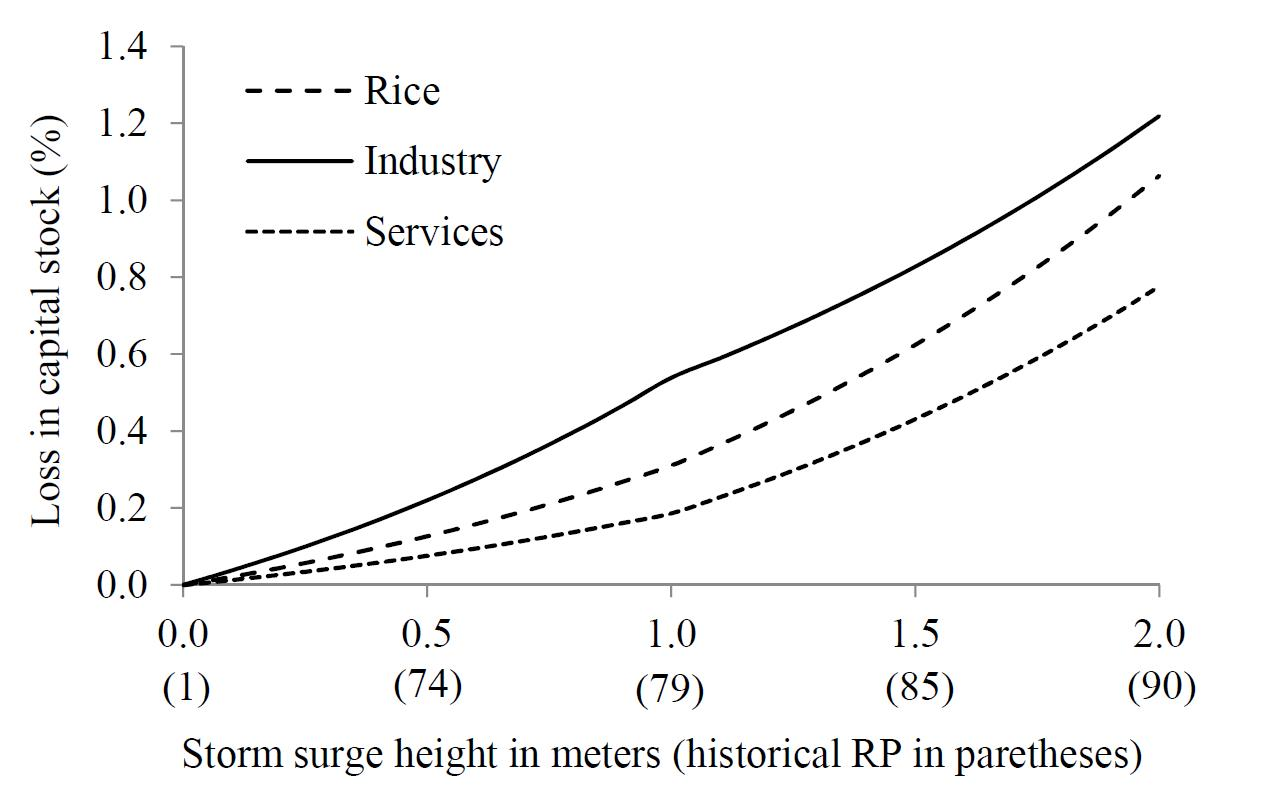
\includegraphics[width = 8cm, height = 8cm]{pictures/DamagesCyclones.jpg}
\end{center}
\footnotesize{Source: The illustration is published in \cite{arndt2015economic}.}
\end{figure}

\subsection{Adaptation}

One classical example of an adaptation measure against climate change and especially sea level rise are dikes. A dike needs to be build before the sea level rises. A dike is a capital good which needs maintenance. \cite{lenk2017costs} show that construction costs of a dike with one meter length and one meter height is 40,000 EURO. The coastline of the Mekong River Delta is 600 km long. Building a dike along the coastline of the Mekong River Delta of one meter height costs roughly 24 billion Euro or roughly 15\% of the GDP of Vietnam in 2016. We assume that the damage caused by inundation can be reduced to zero if the height of the dike exceeds the change in sea level \eqref{eq:Damages}. Otherwise, the full damage materializes. We can translate the monetary value of the dike into meters, using the estimates by \cite{lenk2017costs}. If sea level rises by one meter the cumulative invesmtents into the dike have to exceed 24 billion Euro excluding maintenance costs.

\subsection{Results}

\cleardoublepage
\section{How to use the model?}\label{sec:modelusage}
\subsection{Usage}
\begin{enumerate}
\item In order to use the model you need to install \href{https://www.dynare.org/download/}{Dynare (at least version 4.6.1)} and \href{https://www.mathworks.com/products/matlab.html}{Matlab (at least 2018b)} or \href{https://www.gnu.org/software/octave/}{Octave} on your computing machine. 
For Octave you need to have the version 5.2.0 as reported by the Dynare team. 
Furthermore, MS Excel is used to specify the parameters and to save the results. Result tables are saved additionally in Latex-format.

\item You need to download the repository from Github. 
\item Open Octave or Matlab GUI and browse to the location of the folder in your computer. You have the right folder if the command {\tt pwd()} returns {\tt YourPath/DGE-CRED/DGE_CRED_Model}.
\item The script {\tt RunSimulations.m} has to be executed in order to run simulations for different scenarios. Make sure that the scenarios and model parameters are defined in the file \\ {\tt ModelSimulationandCalibrationKSectorsandRRegions.xlsx}. 
You need to adopt the number of sectors and regions in the file {\tt DGE\_CRED\_Model.mod}. All program files are described in the next section.
\item The simulation results are stored in the file {\tt ResultsScenariosKSectorsandRRegions.xlsx}.
\end{enumerate}

\subsection{Folder structure}
\begin{enumerate}
\item The main file containing all necessary mod-files is {\tt DGE_CRED_Model.mod}. This file includes the following files stored in the {\tt ModFiles} folder:
\begin{enumerate}
\item {\tt DGE_CRED_Model_Declarations.mod} declares all endogenous and exogenous variables of the model and structural parameters.
\item {\tt DGE_CRED_Model_Parameters.mod} assigns values to the structural parameters of the model.
\item {\tt DGE_CRED_Model_Equations.mod} contains the equations of the model.
\item {\tt DGE_CRED_Model_LatexOutput.mod} produces latex output for documentation of the declared variables and model equations.
\item {\tt DGE_CRED_Model_SteadyState.mod} computes initial and terminal condition for the dynamic simulation.
\item {\tt DGE_CRED_Model_Simulations.mod} starts the dynamic simulation.
\end{enumerate}
\item Subroutines responsible for finding the initial and terminal conditions are located in the subfolder {\tt Functions}:
\begin{enumerate}
\item {\tt Calibration.mat} finds the initial conditions to reflect a specific year of the economy.
\item {\tt FindA.mat} looks for exogenous productivity shocks across sectors and regions to meet the terminal conditions.
\item {\tt FindK.mat} looks for a capital allocation across sectors and regions to fulfill the static equations of the model.
\item {\tt rng.mat} random number generator function necessary for Octave users.
\item {\tt LoadExogenous.mat} reads exogenous variables for different scenarios.
\end{enumerate}
\item To define scenarios and structural parameters you need to create an Excel file located in the subfolder {\tt ExcelFiles}:
\begin{enumerate}
\item {\tt ModelSimulationandCalibrationforKSectorsandRregions.xlsx} has multiple sheets:
\begin{enumerate}
\item initial {\tt Start}
\item terminal {\tt Terminal}
\item parameters to define rigidity parameters {\tt Dynamics}
\item elasticity parameters and tax rates {\tt Structural Parameters}
\item coefficients for regional and sector specific damage functions {\tt Climate Damage Functions (Labour, Capital, TFP)}
\item {\tt Baseline} scenario and other optional scenario sheets {\tt Adaptation and Extremes} defining paths for exogenous variables 
\item {\tt Data} to load external data sources
\end{enumerate}
\item {\tt ResultsScenariosKSectorsandRregions.xlsx} has as many sheets as scenarios defined in the previous Excel file.
\end{enumerate}
\item The latex files produced by {\tt DGE_CRED_Model_LatexOutput.mod} are stored in the sub-folder {\tt LatexFiles}:
\begin{enumerate}
\item the system of dynamic equations as implemented in Matlab {\tt DGE_CRED_Model_Dynamic}, \\
 {\tt DGE_CRED_Model_Dynamic_content}
\item names of endogenous, exogenous variables and parameters {\tt DGE_CRED_Model_latex_definitions}
\item the system of dynamic equations in original form without auxiliary variables for leads and lags {\tt DGE_CRED_Model_original}, {\tt DGE_CRED_Model_original_content}
\end{enumerate}
\item The file to run different simulations is {\tt RunSimulations.m}.
\item A Matlab function to find solutions to the static system of equations is {\tt DGE_CRED_Model_steady_state.m}.
\end{enumerate}

\bibliography{references}
\clearpage
\appendix
\section{Model equations for CRED baseline version}\label{app:modelequationsbaseline}
\footnotesize
% Equation 1
\subsection{Regional Industries}
% Equation 1
damage function TFP
\begin{dmath}
{{D_{k,r}}_{t}}=exp\left(-\phi^{G^{A}_{k,r}} \, G^{A}_{k,r,t}\right) \, \left({{a_{T,1,k,r}}} \, {{T_{r}}_{t}}+{{a_{T,2,k,r}}}\, \left({T_{r}}_{t}\right)^{a_{T,3,k,r}}+{{a_{SL,1,k,r}}}\, {{SL}_{t}}+{{a_{SL,2,k,r}}}\, \left({SL}_{t}\right)^{{{a_{SL,3,k,r}}}}+{{a_{W,1,k,r}}}\, {{W_{r}^{S}}_{t}}+{{a_{W,2,k,r}}}\, \left({W_{r}^{S}}_{t}\right)^{{{a_{W,3,k,r}}}}+{{a_{P,1,k,r}}}\, {{PREC_{r}}_{t}}+{{a_{P,2,k,r}}}\, \left({PREC_{r}}_{t}\right)^{{{a_{P,3,k,r}}}}+{{a_{C,1,k,r}}}\, {{CYC_{r}}_{t}}+{{a_{C,2,k,r}}}\, \left({CYC_{r}}_{t}\right)^{{{a_{C,3,k,r}}}}+{{a_{D,1,k,r}}}\, {{DRO_{r}}_{t}}+{{a_{D,2,k,r}}}\, \left({DRO_{r}}_{t}\right)^{{{a_{DRO,3,k,r}}}}\right) 
\end{dmath}
damage function capital
\begin{dmath}
{{D^{K}_{k,r}}_{t}}=exp\left(-\phi^{G^{A}_{k,r}} \, G^{A}_{k,r,t}\right) \, \left({{a^{K}_{T,1,k,r}}} \, {{T_{r}}_{t}}+{{a^{K}_{T,2,k,r}}}\, \left({T_{r}}_{t}\right)^{a^{K}_{T,3,k,r}}+{{a^{K}_{SL,1,k,r}}}\, {{SL}_{t}}+{{a^{K}_{SL,2,k,r}}}\, \left({SL}_{t}\right)^{{{a^{K}_{SL,3,k,r}}}}+{{a^{K}_{W,1,k,r}}}\, {{W_{r}^{S}}_{t}}+{{a^{K}_{W,2,k,r}}}\, \left({W_{r}^{S}}_{t}\right)^{{{a^{K}_{W,3,k,r}}}}+{{a^{K}_{P,1,k,r}}}\, {{PREC_{r}}_{t}}+{{a^{K}_{P,2,k,r}}}\, \left({PREC_{r}}_{t}\right)^{{{a^{K}_{P,3,k,r}}}}+{{a^{K}_{C,1,k,r}}}\, {{CYC_{r}}_{t}}+{{a^{K}_{C,2,k,r}}}\, \left({CYC_{r}}_{t}\right)^{{{a^{K}_{C,3,k,r}}}}+{{a^{K}_{D,1,k,r}}}\, {{DRO_{r}}_{t}}+{{a^{K}_{D,2,k,r}}}\, \left({DRO_{r}}_{t}\right)^{{{a^{K}_{DRO,3,k,r}}}}\right) 
\end{dmath}
damage function labour productivity
\begin{dmath}
{{D^{N}_{k,r}}_{t}}=exp\left(-\phi^{G^{A}_{k,r}} \, G^{A}_{k,r,t}\right) \, \left({{a^{N}_{T,1,k,r}}} \, {{T_{r}}_{t}}+{{a^{N}_{T,2,k,r}}}\, \left({T_{r}}_{t}\right)^{a^{N}_{T,3,k,r}}+{{a^{N}_{SL,1,k,r}}}\, {{SL}_{t}}+{{a^{N}_{SL,2,k,r}}}\, \left({SL}_{t}\right)^{{{a^{N}_{SL,3,k,r}}}}+{{a^{N}_{W,1,k,r}}}\, {{W_{r}^{S}}_{t}}+{{a^{N}_{W,2,k,r}}}\, \left({W_{r}^{S}}_{t}\right)^{{{a^{N}_{W,3,k,r}}}}+{{a^{N}_{P,1,k,r}}}\, {{PREC_{r}}_{t}}+{{a^{N}_{P,2,k,r}}}\, \left({PREC_{r}}_{t}\right)^{{{a^{N}_{P,3,k,r}}}}+{{a^{N}_{C,1,k,r}}}\, {{CYC_{r}}_{t}}+{{a^{N}_{C,2,k,r}}}\, \left({CYC_{r}}_{t}\right)^{{{a^{N}_{C,3,k,r}}}}+{{a^{N}_{D,1,k,r}}}\, {{DRO_{r}}_{t}}+{{a^{N}_{D,2,k,r}}}\, \left({DRO_{r}}_{t}\right)^{{{a^{N}_{DRO,3,k,r}}}}\right) 
\end{dmath}
government expenditure for adaptation measures
\begin{dmath}
G^{A}_{k,r,t}=\eta_{G^{A},k,r,t}
\end{dmath}
% Equation 2
TFP
\begin{dmath}
A_{k,r,t}= A_{k,r,0} \, exp\left({\eta_{A,k,r,t}}\right)
\end{dmath}
% Equation 3
capital specific productivity
\begin{dmath}
A^{K}_{k,r,t}= A^{K}_{k,r,0} \, exp\left({\eta_{A^{K},k,r,t}}\right)
\end{dmath}
% Equation 4
labour specific productivity
\begin{dmath}
A^{N}_{k,r,t}= A^{N}_{k,r,0} \, exp\left({\eta_{A^{N},k,r,t}}\right)
\end{dmath}
% Equation 3
price of regional sectoral goods
\begin{dmath}
\frac{{{P_{k,r}}_{t}}}{{{P_k}_{t}}}={{\omega^{Q}_{k,r}}}^{\frac{1}{{{\eta^{Q}_{k}}}}}\, \left(\frac{{{Y_{k,r}}_{t}}}{{{Y_k}_{t}}}\right)^{\frac{\left(-1\right)}{{{\eta^{Q}_{k}}}}}
\end{dmath}
% Equation 3
production function
\begin{dmath}
{{Y_{k,r}}_{t}}={{A_{k,r}}_{t}}\, \left(1-{{D_{k,r}}_{t}}\right)\, \left({{\alpha^{K}_{k,r}}}^{\frac{1}{{{\eta^{N,K}_{k,r}}}}}\, \left({{A^{K}_{k,r}}_{t}}\, {{K_{k,r}}_{t-1}}\right)^{\frac{{{\eta^{N,K}_{k,r}}}-1}{{{\eta^{N,K}_{k,r}}}}}+{{\alpha^{N}_{k,r}}}^{\frac{1}{{{\eta^{N,K}_{k,r}}}}}\, \left({{A^{N}_{k,r}}_{t}}\, (1 -  {Pop_{t}}\, {{N_{k,r}}_{t}}\right)^{\frac{{{\eta^{N,K}_{k,r}}}-1}{{{\eta^{N,K}_{k,r}}}}}\right)^{\frac{{{\eta^{N,K}_{k,r}}}}{{{\eta^{N,K}_{k,r}}}-1}}
\end{dmath}
% Equation 4
firms FOC capital
\begin{dmath}
{{r_{k,r}}_{t}} \, \left(1+\tau^{K}_{k,r,t}\right)={{\alpha^{K}_{k,r}}}^{\frac{1}{{{\eta^{N,K}_{k,r}}}}}\, {{A^{K}_{k,r}}_{t}}^{\frac{{{\eta^{N,K}_{k,r}}}-1}{{{\eta^{N,K}_{k,r}}}}}\, \left(\frac{{{K_{k,r}}_{t-1}}}{{{Y_{k,r}}_{t}}}\right)^{\frac{-1}{{{\eta^{N,K}_{k,r}}}}}
\end{dmath}
% Equation 5
Firms FOC labour
\begin{dmath}
\frac{{{W_{k,r}}_{t}}\left(1+\tau^{N}_{k,r,t}\right)}{{{P_{k,r}}_{t}}}={{\alpha^{N}_{k,r}}}^{\frac{1}{{{\eta^{N,K}_{k,r}}}}}\, \left(\frac{{{A^{N}_{k,r}}_{t}}\, {Pop_{t}}\, {{N_{k,r}}_{t}}}{{{Y_{k,r}}_{t}}}\right)^{\frac{-1}{{{\eta^{N,K}_{k,r}}}}}
\end{dmath}

\subsection{Aggregation}
relative price of sectoral output
\begin{dmath}
\frac{{{P_k}_{t}}}{{P_{t}}}={{\omega^{Q}_{k}}}^{\frac{1}{{{\eta^{Q}}}}}\, \left(\frac{{{Y_k}_{t}}}{{Y_{t}}}\right)^{\frac{\left(-1\right)}{{{\eta^{Q}}}}}
\end{dmath}
sectoral CES aggregation
\begin{dmath}
{Y_k,t}=\left(\sum_{r}^{R}{{\omega^{Q}_{k,r}}}^{\frac{1}{{{\eta^{Q}_{k}}}}}\, {{Y_{k,r}}_{t}}^{\frac{{{\eta^{Q}_{k}}}-1}{{{\eta^{Q}_{k}}}}}\right)^{\frac{{{\eta^{Q}_{k}}}}{{{\eta^{Q}_{k}}}-1}}
\end{dmath}


\subsection{Households}
% Equation 6
households FOC labour
\begin{dmath}
\frac{{{W_{k,r}}_{t}}\, \left(1-{{\tau^{N}}}\right)\, \left(\frac{{C_{t}}}{{Pop_{t}}}\right)^{\left(-{{\sigma^{C}}}\right)}}{\left(1+{{\tau^{C}}}\right) \, P_{t}}={{\phi^{L}}}\, {{N_k}_{t}}^{{{\sigma^{L}}}}
\end{dmath}
% Equation 7
households FOC capital
\begin{dmath}
\frac{\left(\frac{{P_{t+1}}\, {C_{t+1}}}{{Pop_{t+1}}}\right)^{\left(-{{\sigma^{C}}}\right)}}{\left(1+{{\tau^{C}}}\right) \, P_{t+1}}\, {{\beta}}\, {{P_{k,r}}_{t+1}}\, {{r_{k,r}}_{t+1}}\, \left(1-{{\tau^{K}}}\right)+{{\beta}}\, {{\omega^I_{k,r}}_{t+1}}\, \left(1-{{\delta}}\right)={{\omega^I_{k,r}}_{t}}
\end{dmath}
% Equation 8
households FOC investment
\begin{dmath}
P_{k,r,t}\, \frac{\left(\frac{{C}_{t}}{{Pop}_{t}}\right)^{\left(-{{\sigma^{C}}}\right)}}{{P}_{t}\, \left(1+{{\tau^{C}}}\right)}={{\omega^I_{k,r}}}_{t} \, \frac{\left(\frac{{C}_{t}}{{Pop}_{t}}\right)^{\left(-{{\sigma^{C}}}\right)}}{{P}_{t}\, \left(1+{{\tau^{C}}}\right)}\, \left(S\left(\frac{{{I_{k,r}}}_{t}}{{{I_{k,r}}}_{t-1}}\right) - S'\left(\frac{{{I_{k,r}}}_{t}}{{{I_{k,r}}}_{t-1}}\right) \, \left(\frac{{{I_{k,r}}}_{t}}{{{I_{k,r}}}_{t-1}}\right) \right) + {{\omega^I_{k,r}}}_{t+1}\, \frac{\left(\frac{{C}_{t+1}}{{Pop}_{t+1}}\right)^{\left(-{{\sigma^{C}}}\right)}\, {{\beta}}}{\left(1+{{\tau^{C}}}\right)\, {P}_{t+1}} \, S'\left(\frac{{{I_{k,r}}}_{t+1}}{{{I_{k,r}}}_{t}}\right) \, \frac{{{I_{k,r}}}_{t+1}^{2}}{{{I_{k,r}}}_{t}^{2}}
\end{dmath}
% Equation 8
households LOM capital
\begin{dmath}
{{K_{k,r}}_{t}}={{K_{k,r}}_{t-1}}\, \left(1-{{\delta}}\right) + I_{k,r,t} \, S\left(\frac{{{I_{k,r}}_{t}}}{{{I_{k,r}}_{t-1}}}\right)
\end{dmath}
households FOC foreign bonds
\begin{dmath}
\frac{\left(\frac{{C}_{t+1}}{{Pop}_{t+1}}\right)^{\left(-{{\sigma^{C}}}\right)}}{\left(1+{{\tau^{C}}}\right)\, {P}_{t+1}}\, {{\beta}}\, {S^{f}}_{t+1}\, \exp\left(-\phi^{B}\, \left(\frac{{B}_{t}\, {S^{f}}_{t+1}\, {{r^{f}}}_{t+1}}{{Y}_{t+1}}+\frac{{NX}_{t}}{{Y}_{t}}\right)\right)\, \left(1+{{r^{f}}}_{t+1}\right)=\frac{\left(\frac{{C}_{t}}{{Pop}_{t}}\right)^{\left(-{{\sigma^{C}}}\right)}}{{P}_{t}\, \left(1+{{\tau^{C}}}\right)}
\end{dmath}

\subsection{Climate Variables}
temperature
\begin{dmath}
{{T_{r}}_{t}}={{T_{0,r}}}+{{\eta_{T,r}}_{t}}
\end{dmath}
wind speed
\begin{dmath}
{{W_{r}^{S}}_{t}}={{W^{S}_{0,r}}}+{{\eta_{W^{S},r}}_{t}}
\end{dmath}
precipitation
\begin{dmath}
{{PREC_{r}}_{t}}={{PREC_{0,r}}}+{{\eta_{PREC,r}}_{t}}
\end{dmath}
sea level
\begin{dmath}
{{SL}_{t}}={{SL_0}}+{{\eta_{SL}}_{t}}
\end{dmath}

\subsection{Trade}
trade balance
\begin{dmath}
{NX_{t}}=-\left({B_{t}}-\left(1+{{r^{f}}_{t}}\right) \, S^{f}_{t} \, {B_{t-1}}\right)
\end{dmath}
net exports
\begin{dmath}
{NX_{t}}={{\rho^{NX}}}\, {NX_{t-1}}+{Y_{t}}\, \left(1-{{\rho^{NX}}}\right)\, exp\left({{\eta_{NX}}_{t}}\right)\, {{\omega^{NX}}}
\end{dmath}
foreign interest rates
\begin{dmath}
r^{f}_{t} = \bar{r}^{f}
\end{dmath}

\subsection{Government}
budget constraint
\begin{dmath}
{P_{t}}\, {G_{t}} + \sum_{r}^{R} \sum_{k}^{K} {P_{t}} \, G^{A}_{k,r,t} + {P_{t}} \, {S^{f}_{t}} \, \left(1+{{r^{f}}_{t}}\right)\, {BG_{t-1}}={P_{t}}\, {BG_{t}}+{C_{t}}\, {P_{t}}\, {{\tau^{C}}}+\sum_{k}^{K} \sum_{r}^{R} \, N_{k,r,t} \, W_{k,r,t} \, \left({\tau^{N} + \tau^{N}_{k,r,t}}\right)+{{K_{k,r}}_{t}}\, {{r_{k,r}}_{t}}\, {{P_{k,r}}_{t}}\, \left(\tau^{K} + \tau^{K}_{k,r,t}\right)
\end{dmath}
government foreign debt
\begin{dmath}
{BG_{t}}={{\eta_{BG}}_{t}}
\end{dmath}
tax rates on capital expenditure
\begin{dmath}
\tau^{K}_{k,r,t} = \tau^{K}_{k,r,0} + \eta^{\tau^{K}}_{k,r,t}
\end{dmath}
tax rates on labour compensation
\begin{dmath}
\tau^{N}_{k,r,t} = \tau^{N}_{k,r,0} + \eta^{\tau^{N}}_{k,r,t}
\end{dmath}


\subsection{Aggregates}
national price level
\begin{dmath}
{P_{t}}=exp\left({{\eta_{P}}_{t}}\right)
\end{dmath}
national Population
\begin{dmath}
{PoP_{t}}={{\rho^{Pop}}}\, {Pop_{t-1}}+\left(1-{{\rho^{Pop}}}\right)\, {{Pop_0}}\, exp\left({{\eta_{Pop}}_{t}}\right)
\end{dmath}
resource constraint
\begin{dmath}
{Y_{t}}={C_{t}}+{I_{t}}+{G_{t}}+\sum_{k}^{K} \sum_{r}^{R} {G^{A}_{k,r,t}} + {NX_{t}}
\end{dmath}
sector labour
\begin{dmath}
{{N_k}_{t}}={\sum_{r}^{R} {N_{k,r}}_{t}}
\end{dmath}
sector wage bill
\begin{dmath}
{{N_k}_{t}}\, {{W_k}_{t}}={\sum_{r}^{R} {N_{k,r}}_{t}}\, {{W_{k,r}}_{t}}
\end{dmath}
sector investment
\begin{dmath}
{{P_k}_{t}}\, {{I_k}_{t}}={\sum_{r}^{R} {P_{k,r}}_{t}}\, {{I_{k,r}}_{t}}
\end{dmath}
sector capital stock
\begin{dmath}
{{P_k}_{t}}\, {{K_k}_{t}}={\sum_{r}^{R} {P_{k,r}}_{t}}\, {{K_{k,r}}_{t}}
\end{dmath}
national investment
\begin{dmath}
{P_{t}}\, {I_{t}}={\sum_{k}^{K} {P_k}_{t}}\, {{I_k}_{t}}
\end{dmath}
national capital
\begin{dmath}
{P_{t}}\, {K_{t}}={\sum_{k}^{K} {P_k}_{t}}\, {{K_k}_{t-1}}
\end{dmath}
national output
\begin{dmath}
{P_{t}}\, {Y_{t}}={\sum_{k}^{K} {P_k}_{t}}\, {{Y_k}_{t}}
\end{dmath}
national labour share
\begin{dmath}
{N_{t}}={\sum_{k}^{K} {N_k}_{t}}
\end{dmath}
\section{Additional and modified model equations for input-output extension}\label{app:modelequationsextension1}
\footnotesize
% Equation 1
\subsection{Regional Industries}
% Equation 3
demand for regional sector output
\begin{dmath}
\frac{{{P^{D}_{k,r}}_{t}}}{{{P^{D}_k}_{t}}}={{\omega^{Q}_{k,r}}}^{\frac{1}{{{\eta^{Q}_{k}}}}}\, \left(\frac{{{Q_{k,r}}_{t}}}{{{Q_k}_{t}}}\right)^{\frac{\left(-1\right)}{{{\eta^{Q}_{k}}}}}
\end{dmath}
% Equation 3
output production function
\begin{dmath}
{{Q_{k,r}}_{t}}= \left({{\omega^{Q^{I}}_{k,r}}}^{\frac{1}{{{\eta^{I}_{k,r}}}}}\, \left(Q^{I}_{k,r,t}\right)^{\frac{{{\eta^{Q^{I}}_{k,r}}}-1}{{{\eta^{Q^{I}}_{k,r}}}}}+\left(1 - {{\omega^{Q^{I}}_{k,r}}} \right)^{\frac{1}{{{\eta^{I}_{k,r}}}}} \, \left(Y_{k,r,t}\right)^{\frac{{{\eta^{I}_{k,r}}}-1}{{{\eta^{I}_{k,r}}}}}\right)^{\frac{{{\eta^{I}_{k,r}}}}{{{\eta^{I}_{k,r}}}-1}}
\end{dmath}
% Equation 4
demand for gross value added products
\begin{dmath}
\frac{{{P_{k,r}}_{t}}}{{P^{D}_{k,r,t}}}=\left(1 - {\omega^{Q^{I}}_{k,r}}\right)^{\frac{1}{{{\eta^{I}_{k}}}}} \, \left(\frac{Y_{k,r,t}}{Q_{k,r,t}}\right)^{\frac{\left(-1\right)}{{{\eta^{I}_{k}}}}}
\end{dmath}
% Equation 4
demand for intermediate products
\begin{dmath}
\frac{{P_{t}}}{{P^{D}_{k,r,t}}}={\omega^{Q^{I}}_{k,r}}^{\frac{1}{{{\eta^{I}_{k}}}}} \, \left(\frac{Q^{I}_{k,r,t}}{Q_{k,r,t}}\right)^{\frac{\left(-1\right)}{{{\eta^{I}_{k}}}}}
\end{dmath}

\subsection{Aggregation}
demand for domestically used sectoral products
\begin{align}
\frac{P^{D}_{k,t}}{P^{D}_{t}}={{\omega^{Q}_{k}}}^{\frac{1}{{{\eta^{Q}}}}}\, \left(\frac{Q^{D}_{k,t}}{{Q^{D}_{t}}}\right)^{\frac{\left(-1\right)}{{{\eta^{Q}}}}} \label{eq:demandsectoraloutput}
\end{align}
use of domestically produced products
\begin{align}
Q_{k,t} = Q^{D}_{k,t} + X_{k,t}
\end{align}
sectoral CES aggregation
\begin{align}
Q_{k,t}=\left(\sum_{r}^{R}{{\omega^{Q}_{k,r}}}^{\frac{1}{{{\eta^{Q}_{k}}}}}\, {{Q_{k,r}}_{t}}^{\frac{{{\eta^{Q}_{k}}}-1}{{{\eta^{Q}_{k}}}}}\right)^{\frac{{{\eta^{Q}_{k}}}}{{{\eta^{Q}_{k}}}-1}}
\end{align}
demand for domestically used and produced products
\begin{align}
\frac{P^{D}_{t}}{P_{t}}={(1 - \omega^{F})}^{\frac{1}{{{\eta^{F}}}}}\, \left(\frac{Q^{D}_{t}}{{Q^{U}_{t}}}\right)^{\frac{\left(-1\right)}{{{\eta^{F}}}}} \label{eq:demanddomesticoutput}
\end{align}
demand for imports
\begin{align}
\frac{P^{M}_{t}}{P_{t}}={(\omega^{F})}^{\frac{1}{{{\eta^{F}}}}}\, \left(\frac{M_{t}}{{Q^{U}_{t}}}\right)^{\frac{\left(-1\right)}{{{\eta^{F}}}}} \label{eq:demandimports}
\end{align}
demand for sectoral imports
\begin{align}
\frac{P^{M}_{k,t}}{P^{M}_{t}}={(\omega^{F})}^{\frac{1}{{{\eta^{F}}}}}\, \left(\frac{M_{k,t}}{{M_{t}}}\right)^{\frac{\left(-1\right)}{{{\eta^{F}}}}} \label{eq:demandsectoralimports}
\end{align}

\subsection{Aggregates}
resource constraint
\begin{align}
\frac{P^{D}_t}{P_t} \, Q_{t} = C_{t} + I_{t} + G_{t} + \sum_{k}^{K} \sum_{r}^{R} {G^{A}_{k,r,t}} + Q^{I}_{t} + {NX_{t}} \label{eq:resourceconstraint}
\end{align}
total demand for intermediate products
\begin{align}
P_{t} Q^{I}_{t} = \sum_{k}^{K} \sum_{r}^{R} P_{t} \, Q^{I}_{k,r,t}
\end{align}
total sectoral demand for intermediate products
\begin{align}
P_{t} Q^{I}_{k,t} = \sum_{r}^{R} P_{t} \, Q^{I}_{k,r,t}
\end{align}
definition of domestically used and produced products
\begin{align}
P^{D}_{t} \, Q^{D}_{t} = \sum_{k} P^{D}_{k,t} \, Q^{D}_{k,t}
\end{align}
definition of domestic output
\begin{align}
P_{t} \, Q_{t} = \sum_{k}^{K} P^{D}_{k,t} \, Q^{D}_{k,t}
\end{align}
definition of domestically used products
\begin{align}
P_{t} \, Q^{U}_{t} = P^{M}_{t} \, M_{t} + P^{D}_{t} \, Q^{D}_{t}
\end{align}
exports
\begin{align}
P^{D}_{t} X_{t} = \sum_{k}^{K} P^{D}_{k,t} \, X_{k,t}
\end{align}
imports
\begin{align}
P^{M}_{t} M_{t} = \sum_{k}^{K} P^{M}_{k,t} \, M_{k,t}
\end{align}
net exports
\begin{align}
P_{t} NX_{t} = P^{D}_{t} \, X_{t} - P^{M}_{t} \, M_{t} \label{eq:netexports}
\end{align}

\subsection{Trade}
demand for sectoral exports
\begin{align}
{X_{k,t}} = D^{X}_{k,t} \, Q_{k,t} \nonumber \\
D^{X}_{k,t} = D^{X}_{k,0} + \eta^{X}_{k,t} \label{eq:exportsdemand}
\end{align}
price for sectoral imports
\begin{align}
P^{M}_{k,t} = P^{M}_{k,0} + \eta^{M}_{k,t} \label{eq:importprices}
\end{align}


\section{Additional and modified model equations for energy extension}\label{app:modelequationsextension2}
\footnotesize
% Equation 1
\subsection{Regional Energy industries}
% Equation 3
output production function
\begin{dmath}
{{Q_{k,r}}_{t}}= \left({{\omega^{Q^{I}}_{k,r}}}^{\frac{1}{{{\eta^{I}_{k,r}}}}}\, \left(Q^{I,E}_{k,r,t}\right)^{\frac{{{\eta^{Q^{I}}_{k,r}}}-1}{{{\eta^{Q^{I}}_{k,r}}}}}+\left(1 - {{\omega^{Q^{I}}_{k,r}}} \right)^{\frac{1}{{{\eta^{I}_{k,r}}}}} \, \left(Y_{k,r,t}\right)^{\frac{{{\eta^{I}_{k,r}}}-1}{{{\eta^{I}_{k,r}}}}}\right)^{\frac{{{\eta^{I}_{k,r}}}}{{{\eta^{I}_{k,r}}}-1}}
\end{dmath}
nested composition function for intermediate energy and non-energy inputs
\begin{dmath}
{{Q^{I,E}_{k,r}}_{t}}= \left(({1-\omega^{Q^{E}}_{k,r}})^{\frac{1}{{{\eta^{E}_{k,r}}}}} \, \left(Q^{I,E}_{k,r,t}\right)^{\frac{{{\eta^{E}_{k,r}}}-1}{{{\eta^{E}}_{k,r}}}}+\left(\omega^{E}_{k,r} \right)^{\frac{1}{{{\eta^{E}_{k,r}}}}} \, \left(E_{k,r,t}\right)^{\frac{{{\eta^{E}_{k,r}}}-1}{{{\eta^{E}_{k,r}}}}}\right)^{\frac{{{\eta^{E}_{k,r}}}}{{{\eta^{E}_{k,r}}}-1}} \label{eq:energyintermediatecomposite}
\end{dmath}
nested composition function for energy inputs
\begin{dmath}
E_{k,r,t}= \left( \sum_{c}^{EC} {\omega^{Q^{E}}_{k,r,c}}^{\frac{1}{{{\eta^{EC}_{k,r}}}}}\, \left(E_{k,r,c,t}\right)^{\frac{{{\eta^{EC}_{k,r}}}-1}{{{\eta^{EC}}_{k,r}}}}\right)^{\frac{{{\eta^{EC}_{k,r}}}}{{{\eta^{EC}_{k,r}}}-1}} \label{eq:energycomposite}
\end{dmath}
demand for intermediate products
\begin{dmath}
\frac{{P^{I}_{k,r,t}}}{{P^{D}_{k,r,t}}}={\omega^{Q^{I}}_{k,r}}^{\frac{1}{{{\eta^{I}_{k}}}}} \, \left(\frac{Q^{I}_{k,r,t}}{Q^{I,E}_{k,r,t}}\right)^{\frac{\left(-1\right)}{{{\eta^{I}_{k}}}}}
\end{dmath}
demand for energy as intermediate product
\begin{dmath}
\frac{{P^{E}_{k,r,t}}}{{P^{I}_{k,r,t}}}={\omega^{E}_{k,r}}^{\frac{1}{{{\eta^{E}_{k,r}}}}} \, \left(\frac{E_{k,r,t}}{Q^{I,E}_{k,r,t}}\right)^{\frac{\left(-1\right)}{{{\eta^{E}_{k}}}}}
\end{dmath}
demand for non-energy intermediate products
\begin{dmath}
\frac{P_{t}}{P^{I}_{k,r,t}} = (1 - \omega^{E}_{k,r})^{\frac{1}{{{\eta^{E}_{k,r}}}}} \, \left(\frac{Q^{I}_{k,r,t}}{Q^{I,E}_{k,r,t}}\right)^{\frac{\left(-1\right)}{{{\eta^{E}_{k}}}}}
\end{dmath}


\subsection{Aggregates}
total demand for intermediate products
\begin{align}\label{eq:aggregationintermediateinputswithenergy}
P_{t} Q^{I}_{t} = \sum_{k}^{K} \sum_{r}^{R} \begin{cases}
			P^{I}_{k,r,t} \, Q^{I,E}_{k,r,t} & \mbox{if} k = k^{E} \\
			P_{t} \, Q^{I}_{k,r,t} & \mbox{otherwise}
			\end{cases}
\end{align}

total consumption of energy carrier
\begin{align}
E_{c,t} = \sum_{r}^{R} E_{k^{E},r,c,t} \label{eq:energycarrieraggregate}
\end{align}

price of energy carrier
\begin{align}
P^{EC}_{c,t} = P^{EC}_{c,0} + \eta^{EC}_{c,t} \label{eq:priceenergycarrier}
\end{align}



\cleardoublepage
\begin{center}
\begin{longtable}{lrl}
\caption{List of symbols for baseline version}\label{tab:listofsymbols}\\%
\hline
\multicolumn{1}{c}{\textbf{Variable}} &
\multicolumn{1}{c}{\textbf{\LaTeX}} &
\multicolumn{1}{c}{\textbf{Description}}\\%
\hline\hline%
\endfirsthead
\multicolumn{3}{c}{{\tablename} \thetable{} -- Continued}\\%
\hline%
\multicolumn{1}{c}{\textbf{Variable}} &
\multicolumn{1}{c}{\textbf{\LaTeX}} &
\multicolumn{1}{c}{\textbf{Description}}\\%
\hline\hline%
\endhead
\hline
\multicolumn{3}{c}{Endogenous}\\%
\hline%
\texttt{P} & $P$ & price level\\
\texttt{K} & $K$ & capital stock\\
\texttt{C} & $C$ & consumption\\
\texttt{PoP} & $Pop$ & population\\
\texttt{B} & $B$ & international traded bonds\\
\texttt{Sf} & $S^{f}$ & effective exchange rate with the rest of the world\\
\texttt{BG} & $BG$ & government debt\\
\texttt{NX} & $NX$ & net exports\\
\texttt{rf} & ${r^{f}}$ & foreign interest rate\\
\texttt{G} & $G$ & government expenditure\\
\texttt{I} & $I$ & private investment\\
\texttt{Y} & $Y$ & GDP\\
\texttt{N} & $N$ & labour\\
\texttt{SL} & ${SL}$ & sea level\\
\texttt{PREC\_r} & ${PREC_{r}}$ & regional precipitation\\
\texttt{T\_r} & ${T_{r}}$ & regional temperature\\
\texttt{WS\_r} & ${W_{r}^{S}}$ & regional wind speed\\
\texttt{Y\_k} & ${Y_k}$ & sector GDP\\
\texttt{K\_k} & ${K_k}$ & sector capital\\
\texttt{N\_k} & ${N_k}$ & sector employment\\
\texttt{I\_k} & ${I_k}$ & sector private investment\\
\texttt{P\_k} & ${P_k}$ & sector price index\\
\texttt{W\_k} & ${W_k}$ & sector wage index\\
\texttt{Y\_k\_r} & ${Y_{k,r}}$ & regional sector GDP\\
\texttt{D\_k\_r} & ${D_{k,r}}$ & regional sector damages\\
\texttt{K\_k\_r} & ${K_{k,r}}$ & regional sector capital\\
\texttt{N\_k\_r} & ${N_{k,r}}$ & regional sector employment\\
\texttt{W\_k\_r} & ${W_{k,r}}$ & regional sector wages\\
\texttt{A\_k\_r} & ${A_{k,r}}$ & regional sector TFP\\
\texttt{K\_A\_SL\_k\_r} & ${K^{A,SL}_{k,r}}$ & regional sector capital adaptation stock against sea level\\
\texttt{K\_A\_WS\_k\_r} & ${K^{A,WS}_{k,r}}$ & regional sector capital adaptation stock against wind speed\\
\texttt{K\_A\_T\_k\_r} & ${K^{A,T}_{k,r}}$ & regional sector capital adaptation stock against temperature\\
\texttt{K\_A\_PREC\_k\_r} & ${K^{A,PREC}_{k,r}}$ & regional sector capital adaptation stock against precipitation\\
\texttt{K\_A\_CYC\_k\_r} & ${K^{A,CYC}_{k,r}}$ & regional sector capital adaptation stock against cyclones\\
\texttt{K\_A\_DRO\_k\_r} & ${K^{A,DRO}_{k,r}}$ & regional sector capital adaptation stock against droughts\\
\texttt{G\_A\_SL\_k\_r} & ${G^{A,SL}_{k,r}}$ & regional sector adaptation government expenditure against sea level\\
\texttt{G\_A\_T\_k\_r} & ${G^{A,T}_{k,r}}$ & regional sector adaptation government expenditure against temperature\\
\texttt{G\_A\_WS\_k\_r} & ${G^{A,WS}_{k,r}}$ & regional sector adaptation government expenditure against wind speed\\
\texttt{G\_A\_PREC\_k\_r} & ${G^{A,PREC}_{k,r}}$ & regional sector adaptation government expenditure against precipitation\\
\texttt{G\_A\_CYC\_k\_r} & ${G^{A,CYC}_{k,r}}$ & regional sector adaptation government expenditure against cyclones\\
\texttt{G\_A\_DRO\_k\_r} & ${G^{A,DRO}_{k,r}}$ & regional sector adaptation government expenditure against droughts\\
\texttt{gA\_k\_r} & ${g^{A}_{k,r}}$ & regional growth rate of sector TFP\\
\texttt{A\_N\_k\_r} & ${A^{N}_{k,r}}$ & regional sector labour specific TFP\\
\texttt{A\_K\_k\_r} & ${A^{K}_{k,r}}$ & regional sector capital specific TFP\\
\texttt{I\_k\_r} & ${I_{k,r}}$ & regional sector private investment\\
\texttt{P\_k\_r} & ${P_{k,r}}$ & regional sector price index\\
\texttt{omegaI\_k\_r} & ${\omega^I_{k,r}}$ & shadow value of regional private sector investment\\
\texttt{r\_k\_r} & ${r_{k,r}}$ & regional sector rental rate on capital\\
\texttt{tauKF\_k\_r} & ${\tau^{K,F}_{k,r}}$ & regional sector corporate tax rate on capital firms\\
\texttt{tauNF\_k\_r} & ${\tau^{N,F}_{k,r}}$ & regional sector labour tax rate on capital firms\\
\texttt{tauKH} & ${\tau^{K,H}}$ & tax rate on capital households\\
\texttt{tauNH} & ${\tau^{N,H}}$ & tax rate on clabour income households\\
\hline
\multicolumn{3}{c}{Exogenous}\\%
\hline
\texttt{exo\_P} & ${\eta_{P}}$ & exogenous price index evolution\\
\texttt{exo\_PoP} & ${\eta_{Pop}}$ & exogenous population\\
\texttt{exo\_rf} & ${\eta_{r^f}}$ & exogenous world interest rate\\
\texttt{exo\_SL} & ${\eta_{SL}}$ & exogenous sea level\\
\texttt{exo\_NX} & ${\eta_{NX}}$ & exogenous net exports\\
\texttt{exo\_BG} & ${\eta_{BG}}$ & exogenous structural balance\\
\texttt{exo\_tauKF\_k\_r} & ${\eta_{\tau^{K,F},k,r}}$ & exogenous sector and region corporate tax rate\\
\texttt{exo\_tauNF\_k\_r} & ${\eta_{\tau^{N,F},k,r}}$ & exogenous sector and region labour tax rate\\
\texttt{exo\_tauKH} & ${\eta_{\tau^{K,H}}}$ & exogenous capital income tax rate households\\
\texttt{exo\_tauNH} & ${\eta_{\tau^{N,H}}}$ & exogenous labour income  tax rate households\\
\texttt{exo\_k\_r} & ${\eta_{A,k,r}}$ & exogenous TFP\\
\texttt{exo\_N\_k\_r} & ${\eta_{A^{N},k,r}}$ & exogenous labour specific TFP\\
\texttt{exo\_K\_k\_r} & ${\eta_{A^{K},k,r}}$ & exogenous capital specific TFP\\
\texttt{exo\_GA\_SL\_k\_r} & ${\eta_{G^{A,SL},k,r}}$ & exogenous sector adaptation government expenditure against sea level\\
\texttt{exo\_GA\_T\_k\_r} & ${\eta_{G^{A,T},k,r}}$ & exogenous sector adaptation government expenditure against temperature\\
\texttt{exo\_GA\_WS\_k\_r} & ${\eta_{G^{A,SL},k,r}}$ & exogenous sector adaptation government expenditure against wind speed\\
\texttt{exo\_GA\_PREC\_k\_r} & ${\eta_{G^{A,SL},k,r}}$ & exogenous sector adaptation government expenditure against precipitation\\
\texttt{exo\_GA\_CYC\_k\_r} & ${\eta_{G^{A,SL},k,r}}$ & exogenous sector adaptation government expenditure against cyclones\\
\texttt{exo\_GA\_DRO\_k\_r} & ${\eta_{G^{A,SL},k,r}}$ & exogenous sector adaptation government expenditure against drought\\
\texttt{exo\_T\_r} & ${\eta_{T,r}}$ & exogenous regional temperature\\
\texttt{exo\_PREC\_r} & ${\eta_{PREC,r}}$ & exogenous regional precipitation\\
\texttt{exo\_WS\_r} & ${\eta_{WS,r}}$ & exogenous regional wind speed\\
\hline%
\multicolumn{3}{c}{Parameters}\\%
\hline%
\texttt{omegaQ\_k\_p} & ${\omega^{Q}_{k}}$ & distribution parameter for output from one sector\\
\texttt{etaQ\_k\_p} & ${\eta^{C}_{k}}$ & elasticity of substitution between regional production\\
\texttt{tauK\_k\_r\_p} & ${\tau^{K}_{k,r}}$ & region and sector specific tax rate on capital\\
\texttt{tauN\_k\_r\_p} & ${\tau^{N}_{k,r}}$ & region and sector specific tax rate on labour\\
\texttt{rhoA\_k\_r\_p} & ${\rho^{A}_{k,r}}$ & persistence productivity shock\\
\texttt{rhoA\_N\_k\_r\_p} & ${\rho^{A,N}_{k,r}}$ & persistence labour specific productivity shock\\
\texttt{rhoA\_K\_k\_r\_p} & ${\rho^{A,K}_{k,r}}$ & persistence capital specific productivity shock\\
\texttt{phiY\_k\_r\_p} & $\frac{P_{k,r,0} \, Y_{k,r,0}}{P_{0} \, Y_{0}}$ & long-run share of regional and sectoral output\\
\texttt{phiN\_k\_r\_p} & ${N_{k,r,0}}$ & long-run share of regional and sectoral employment\\
\texttt{phiY0\_k\_r\_p} & $\frac{P_{k,r,0} \, Y_{k,r,0}}{P_{0} \, Y_{0}}$ & terminal share of regional and sectoral output\\
\texttt{phiN0\_k\_r\_p} & ${N_{k,r,0}}$ & initial share of regional and sectoral employment\\
\texttt{phiYT\_k\_r\_p} & $\frac{P_{k,r,0} \, Y_{k,r,0}}{P_{0} \, Y_{0}}$ & terminal share of regional and sectoral output\\
\texttt{phiNT\_k\_r\_p} & ${N_{k,r,0}}$ & terminal share of regional and sectoral employment\\
\texttt{phiW\_k\_r\_p} & $\frac{W_{k,r,0} \, N_{k,r,0}}{P_{k,r,0} \, Y_{k,r,0}}$ & share of regional and sectoral employment\\
\texttt{phiP\_k\_r\_p} & $\frac{P_{k,r,0}}{P_{0}}$ & share of regional and sectoral employment\\
\texttt{phiL\_k\_r\_p} & ${\phi^{L}_{k,r}}$ & coefficient of disutility to work\\
\texttt{omegaQ\_k\_r\_p} & ${\omega^{Q}_{k,r}}$ & distribution parameter for regional production\\
\texttt{alphaK\_k\_r\_p} & ${\alpha^{K}_{k,r}}$ & distribution parameter capital share\\
\texttt{alphaN\_k\_r\_p} & ${\alpha^{N}_{k,r}}$ & distribution parameter labour share\\
\texttt{etaNK\_k\_r\_p} & ${\eta^{N,K}_{k,r}}$ & elasticity of substitution between labour and capital\\
\texttt{A\_k\_r\_p} & ${A_{k,r}}$ & sector long-run TFP\\
\texttt{phiGAT\_k\_r\_p} & ${\phi^{G^{A,T}}_{k,r}}$ & effectiveness of adaptation measures against temperature\\
\texttt{phiGASL\_k\_r\_p} & ${\phi^{G^{A,SL}}_{k,r}}$ & effectiveness of adaptation measures against sea level\\
\texttt{phiGAWS\_k\_r\_p} & ${\phi^{G^{A,WS}}_{k,r}}$ & coefficient of adaptation measures against wind speed\\
\texttt{phiGAPREC\_k\_r\_p} & ${\phi^{G^{A,PREC}}_{k,r}}$ & coefficient of adaptation measures against precipitation\\
\texttt{phiGACYC\_k\_r\_p} & ${\phi^{G^{A,CYC}}_{k,r}}$ & coefficient of adaptation measures against cyclones\\
\texttt{phiGADRO\_k\_r\_p} & ${\phi^{G^{A,DRO}}_{k,r}}$ & coefficient of adaptation measures against droughts\\
\texttt{gY0\_k\_r\_p} & ${\frac{Y_{2,k,r}}{Y_{1,k,r}}}$ & initial sector growth\\
\texttt{gN0\_k\_r\_p} & $\frac{\frac{N_{2,k,r}}{N_{2}}}{\frac{N_{1,k,r}}{N_{1}}}$ & initial sector labour growth\\
\texttt{omegaA\_k\_r\_p} & ${\omega^{A}_{k,r}}$ & exponent for productivity growth\\
\texttt{A\_N\_k\_r\_p} & ${A^{N}_{k,r}}$ & sector labour specific TFP\\
\texttt{A\_K\_k\_r\_p} & ${A^{K}_{k,r}}$ & sector capital specific TFP\\
\texttt{a\_T\_1\_k\_r\_p} & ${a_{1,k,r}}$ & intercept of damage function temperature\\
\texttt{a\_T\_2\_k\_r\_p} & ${a_{2,k,r}}$ & slope of damage function temperature\\
\texttt{a\_T\_3\_k\_r\_p} & ${a_{3,k,r}}$ & exponent of damage function temperature\\
\texttt{a\_PREC\_1\_k\_r\_p} & ${a_{1,k,r}}$ & intercept of damage function precipitation\\
\texttt{a\_PREC\_2\_k\_r\_p} & ${a_{2,k,r}}$ & slope of damage function precipitation\\
\texttt{a\_PREC\_3\_k\_r\_p} & ${a_{3,k,r}}$ & exponent of damage function precipitation\\
\texttt{a\_WS\_1\_k\_r\_p} & ${a_{1,k,r}}$ & intercept of damage function wind speed\\
\texttt{a\_WS\_2\_k\_r\_p} & ${a_{2,k,r}}$ & slope of damage function wind speed\\
\texttt{a\_WS\_3\_k\_r\_p} & ${a_{3,k,r}}$ & exponent of damage function wind speed\\
\texttt{a\_SL\_1\_k\_r\_p} & ${a_{1,k,r}}$ & intercept of damage function sea level\\
\texttt{a\_SL\_2\_k\_r\_p} & ${a_{2,k,r}}$ & slope of damage function sea level\\
\texttt{a\_SL\_3\_k\_r\_p} & ${a_{3,k,r}}$ & exponent of damage function sea level\\
\texttt{a\_CYC\_1\_k\_r\_p} & ${a_{1,k,r}}$ & intercept of damage function cyclone\\
\texttt{a\_CYC\_2\_k\_r\_p} & ${a_{2,k,r}}$ & slope of damage function cyclone\\
\texttt{a\_CYC\_3\_k\_r\_p} & ${a_{3,k,r}}$ & exponent of damage function cyclone\\
\texttt{a\_DRO\_1\_k\_r\_p} & ${a_{1,k,r}}$ & intercept of damage function drought\\
\texttt{a\_DRO\_2\_k\_r\_p} & ${a_{2,k,r}}$ & slope of damage function drought\\
\texttt{a\_DRO\_3\_k\_r\_p} & ${a_{3,k,r}}$ & exponent of damage function drought\\
\texttt{beta\_p} & ${\beta}$ & discount factor\\
\texttt{delta\_p} & ${\delta}$ & capital depreciation rate\\
\texttt{deltaKASL\_k\_r\_p} & ${\delta_{K^{A,SL},k,r}}$ & capital depreciation rate for adaptation capital stock against sea level rise\\
\texttt{deltaKAT\_k\_r\_p} & ${\delta_{K^{A,T},k,r}}$ & capital depreciation rate for adaptation capital stock against temperature\\
\texttt{deltaKAWS\_k\_r\_p} & ${\delta_{K^{A,WS},k,r}}$ & capital depreciation rate for adaptation capital stock against wind speed\\
\texttt{deltaKAPREC\_k\_r\_p} & ${\delta_{K^{A,PREC},k,r}}$ & capital depreciation rate for adaptation capital stock against precipitation\\
\texttt{deltaKACYC\_k\_r\_p} & ${\delta_{K^{A,CYC},k,r}}$ & capital depreciation rate for adaptation capital stock against cyclones\\
\texttt{deltaKADRO\_k\_r\_p} & ${\delta_{K^{A,DRO},k,r}}$ & capital depreciation rate for adaptation capital stock against droughts\\
\texttt{sigmaL\_p} & ${\sigma^{L}}$ & inverse Frisch elasticity\\
\texttt{sigmaC\_p} & ${\sigma^{C}}$ & intertemporal elasticity of substitution\\
\texttt{etaQ\_p} & ${\eta^{Q}}$ & elasticity of substitution between sectoral production\\
\texttt{phiB\_p} & ${\phi^{B}}$ & coefficient of foreign adjustment cost\\
\texttt{phiK\_p} & ${\phi^{K}}$ & coefficient of investment adjustment cost\\
\texttt{tauC\_p} & ${\tau^{C}}$ & consumption tax\\
\texttt{tauNH\_p} & ${\tau^{N}}$ & labour income tax\\
\texttt{tauKH\_p} & ${\tau^{K}}$ & capital income tax\\
\texttt{omegaNX\_p} & ${\omega^{NX}}$ & share of net exports relative to domestic GDP\\
\texttt{omegaNX0\_p} & ${\omega^{NX,0}}$ & initial share of net exports relative to domestic GDP\\
\texttt{omegaNXT\_p} & ${\omega^{NX,T}}$ & terminal share of net exports relative to domestic GDP\\
\texttt{rhoNX\_p} & ${\rho^{NX}}$ & persistency in net exports\\
\texttt{rhoA\_p} & ${\rho^{A}}$ & persistency in TFP\\
\texttt{rhoPoP\_p} & ${\rho^{Pop}}$ & persistency in population\\
\texttt{rhoSL\_p} & ${\rho^{SL}}$ & persistency in sea level\\
\texttt{rhoT\_p} & ${\rho^{T}}$ & persistency in temperature\\
\texttt{rhoWS\_p} & ${\rho^{T}}$ & persistency in wind speed\\
\texttt{rhoPREC\_p} & ${\rho^{T}}$ & persistency in precipitation\\
\texttt{inbsectors\_p} & ${K}$ & number of sectors\\
\texttt{inbregions\_p} & ${R}$ & number of regions\\
\texttt{lCalibration\_p} & ${l^{Calib}}$ & logical indiactor whether model is calibrated or not\\
\texttt{T0\_r\_p} & ${T_{0,n}}$ & initial regional temperature\\
\texttt{PREC0\_r\_p} & ${PREC_{0,n}}$ & initial regional precipitation\\
\texttt{WS0\_r\_p} & ${WS_{0,n}}$ & initial regional wind speed\\
\texttt{TT\_r\_p} & ${T_{T,n}}$ & terminal regional temperature\\
\texttt{PRECT\_r\_p} & ${PREC_{T,n}}$ & terminal regional precipitation\\
\texttt{WST\_r\_p} & ${WS_{T,n}}$ & terminal regional wind speed\\
\texttt{rf0\_p} & ${r^f_0}$ & initial world interest rate\\
\texttt{SL0\_p} & ${SL_0}$ & initial sea level\\
\texttt{PoP0\_p} & ${POP_0}$ & initial population\\
\texttt{Y0\_p} & ${Y_0}$ & initial output\\
\texttt{P0\_p} & ${P_0}$ & initial price level\\
\texttt{N0\_p} & ${N_0}$ & initial employment\\
\texttt{SLT\_p} & ${SL_T}$ & terminal sea level\\
\texttt{PoPT\_p} & ${Pop_T}$ & terminal population\\
\texttt{YT\_p} & ${Y_0}$ & terminal output\\
\texttt{NT\_p} & ${Y_0}$ & terminal employment\\
\hline%
\end{longtable}
\end{center}


\begin{center}
\begin{longtable}{lrr}
\caption{List of symbols for input-output extension}\label{tab:listofsymbolsextension1}\\%
\hline%
\multicolumn{1}{c}{\textbf{Variable}} &
\multicolumn{1}{c}{\textbf{\LaTeX}} &
\multicolumn{1}{c}{\textbf{Description}}\\%
\hline\hline%
\endfirsthead
\multicolumn{3}{c}{{\tablename} \thetable{} -- Continued}\\%
\hline%
\multicolumn{1}{c}{\textbf{Variable}} &
\multicolumn{1}{c}{\textbf{\LaTeX}} &
\multicolumn{1}{c}{\textbf{Description}}\\%
\hline\hline%
\endhead
\hline
\multicolumn{3}{c}{Endogenous}\\%
\hline
\texttt{P\_D} & $P^{D}$ & price level of domestic produced products\\
\texttt{P\_M} & $P^{M}$ & price level of imports\\
\texttt{Q\_U} & $Q^{U}$ & domestic used products \\
\texttt{Q\_D} & $Q^{D}$ & domestic produced and used products\\
\texttt{Q\_I} & $Q^{I}$ & intermediate products\\
\texttt{Q} & $Q$ & doesmtic output\\
\texttt{M} & $M$ & imports\\
\texttt{X} & $X$ & exports\\
\texttt{Q\_k} & ${Q_{k}}$ & sectoral exports\\
\texttt{Q\_D\_k} & ${Q^{D}_{k}}$ & domestic used and produced products\\
\texttt{Q\_I\_k} & ${Q^{I}_{k}}$ & domestic used intermediate products\\
\texttt{M\_k} & ${M_{k}}$ & sectoral imports\\
\texttt{X\_k} & ${X_{k}}$ & sectoral exports\\
\texttt{P\_D\_k} & ${P^{D}_{k}}$ & sectoral price index of domestic products\\
\texttt{P\_M\_k} & ${P^{D}_{k}}$ & sectoral price index of imports\\
\texttt{Q\_k\_r} & ${Q_{k,r}}$ & regional sector output\\
\texttt{Q\_I\_k\_r} & ${Q_{k,r}}$ & regional sector demand for intermediate products\\
\texttt{P\_D\_k\_r} & ${P^{D}_{k,r}}$ & sectoral and regional price index of domestic products\\
\hline
\multicolumn{3}{c}{Exogenous}\\%
\hline
\texttt{exo\_X\_k} & ${\eta^{X}_{k}}$ & exogenous demand for sectoral exports\\
\texttt{exo\_M\_k} & ${\eta^{M}_{k}}$ & exogenous sectoral price of imports\\
\hline
\multicolumn{3}{c}{Parameters}\\%
\hline
\texttt{phiM\_k\_p} & ${\phi^{M}_{k}}$ & initial share of sectoral imports\\
\texttt{phiX\_k\_p} & ${\phi^{X}_{k}}$ & initial share of sectoral exports\\
\texttt{phiQI\_k\_p} & ${\phi^{Q^{I}}_{k}}$ & initial share of sectoral intermediate inputs\\
\texttt{D\_X\_k\_p} & ${D^{X}_{k}}$ & initial demand for sectoral exports\\
\texttt{P\_M\_k\_p} & ${P^{M}_{k}}$ & initial price level for sectoral imports\\
\texttt{omega\_M\_k\_p} & ${\omega^{M}_{k}}$ & distribution parameter for imports\\
\texttt{eta\_I\_k\_p} & ${\eta^{I}_{k}}$ & elasticity of substitution between intermediate products and value added\\
\texttt{omegaQI\_k\_r\_p} & ${\omega^{Q^{I}}_{k,r}}$ & distribution parameter between intermediate products and value added\\
\texttt{etaM\_p} & ${\eta^{M}}$ & elasticity of substitution between sectoral imports\\
\texttt{etaF\_p} & ${\eta^{F}}$ & elasticity of substitution between imports and domestic products\\
\texttt{omegaF\_p} & ${\omega^{F}}$ & distribution parameter for imports\\
\texttt{phiM\_p} & ${\phi^{M}}$ & initial share of imports on toal output\\
\hline%
\end{longtable}
\end{center}


\begin{center}
\begin{longtable}{lrr}
\caption{List of symbols for energy extension}\label{tab:listofsymbolsextension2}\\%
\hline%
\multicolumn{1}{c}{\textbf{Variable}} &
\multicolumn{1}{c}{\textbf{\LaTeX}} &
\multicolumn{1}{c}{\textbf{Description}}\\%
\hline\hline%
\endfirsthead
\multicolumn{3}{c}{{\tablename} \thetable{} -- Continued}\\%
\hline%
\multicolumn{1}{c}{\textbf{Variable}} &
\multicolumn{1}{c}{\textbf{\LaTeX}} &
\multicolumn{1}{c}{\textbf{Description}}\\%
\hline\hline%
\endhead
\hline
\multicolumn{3}{c}{Endogenous}\\%
\hline
\texttt{P\_EC\_c} & $P^{E}_{c}$ & price of energy source\\
\texttt{EC\_c} & $E_{c}$ & consumption of energy source\\
\texttt{E\_k\_r} & $E_{k,r}$ & composite energy consumption \\
\texttt{Q\_IE\_k\_r} & $Q^{I,E}_{k,r}$ & composite intermediate products for energy sector \\
\texttt{P\_I\_k\_r} & $P^{E,Q^{I}}_{k,r}$ & price of composite intermediate products for energy sector \\
\texttt{P\_E\_k\_r} & $P^{E}_{k,r}$ & price of composite energy \\
\texttt{E\_k\_r\_c} & $E_{k,r,c}$ & regional and sectoral consumption of energy source \\
\hline
\multicolumn{3}{c}{Exogenous}\\%
\hline
\texttt{exo\_E\_c} & ${\eta^{E}_{c}}$ & exogenous price for energy source\\
\hline
\multicolumn{3}{c}{Parameters}\\%
\hline
\texttt{phiE\_k\_r\_p} & ${\phi^{E}_{k,r}}$ & initial share of energy on intermediate products\\
\texttt{phiE\_k\_\_r\_c\_p} & ${\phi^{E}_{k,r,c}}$ & initial share of energy source on energy composite intermediate product\\
\texttt{omegaE\_k\_r\_p} & ${\phi^{E}_{k,r}}$ & distribution parameter for energy on intermediate products\\
\texttt{omegaE\_k\_\_r\_c\_p} & ${\phi^{E}_{k,r,c}}$ & distribution parameter for energy source on energy as intermediate product\\
\texttt{etaE\_k\_r\_p} & ${\eta^{E}_{k,r}}$ & elasticity of substitution between energy and other intermediate products\\
\texttt{etaEC\_k\_r\_p} & ${\eta^{E,C}_{k,r}}$ & elasticity of substitution between energy carriers\\
\texttt{P\_EC\_c\_p} & ${P^{E}_{c,0}}$ & initial price for energy source\\
\hline%
\end{longtable}
\end{center}

\end{document}
